\documentclass[xcolor=dvipsnames]{beamer}
\usepackage[T1]{fontenc}
\usepackage[utf8]{inputenc}
\usepackage[english,slovak]{babel}

\usepackage{amsmath}
\usepackage{amsthm}
\usetheme{Pittsburgh}
\useoutertheme{shadow}

\usepackage{graphicx}
\usepackage{caption}
\usepackage{subcaption}

\usepackage[]{algorithm2e}
\usepackage{listings}
 \setbeamercovered{transparent}
 \usepackage{cuted}
\usepackage[export]{adjustbox}



\usepackage{lipsum}

\newcommand\Wider[2][3em]{%
\makebox[\linewidth][c]{%
  \begin{minipage}{\dimexpr\textwidth+#1\relax}
  \raggedright#2
  \end{minipage}%
  }%
}

%-------------------------------------------------------------------------------------
\title{\bf Deep reinforcement learning \\ using sparse distributed memory}
\author{Michal CHOVANEC}


%\setbeamertemplate{footline}[frame number]{}
\setbeamertemplate{navigation symbols}{}



\date[EURP]{\it October 2017}
\begin{document}

\begin{frame}
\titlepage
\end{frame}



\begin{frame}{\bf Overview}

    \begin{itemize}
      \item Reinforcement learning
      \item Sparse representation
      \item Advanced sparse distributed memory
      \item Experimental results
    \end{itemize}


\end{frame}


\begin{frame}{\bf Reinforcement learning}

\centering
Supervised vs. Reinforcement learning

\begin{figure}[htbp]
  \centering
    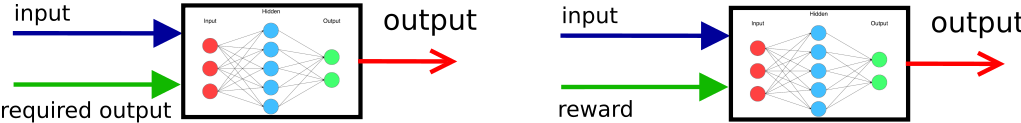
\includegraphics[scale=0.27]{../diagrams/supervised_rl.png}
\end{figure}


\begin{table}[]
\centering
\begin{tabular}{|l|l|l|l|}
\hline
              & input & required output & output \\ \hline
supervised    & yes   & yes             & class  \\ \hline
reinforcement & yes   & unknown         & action \\ \hline
\end{tabular}
\end{table}

\end{frame}


\begin{frame}{\bf Reinforcement learning}

Learning based on rewards and punishments

\begin{figure}[htbp]
  \centering
    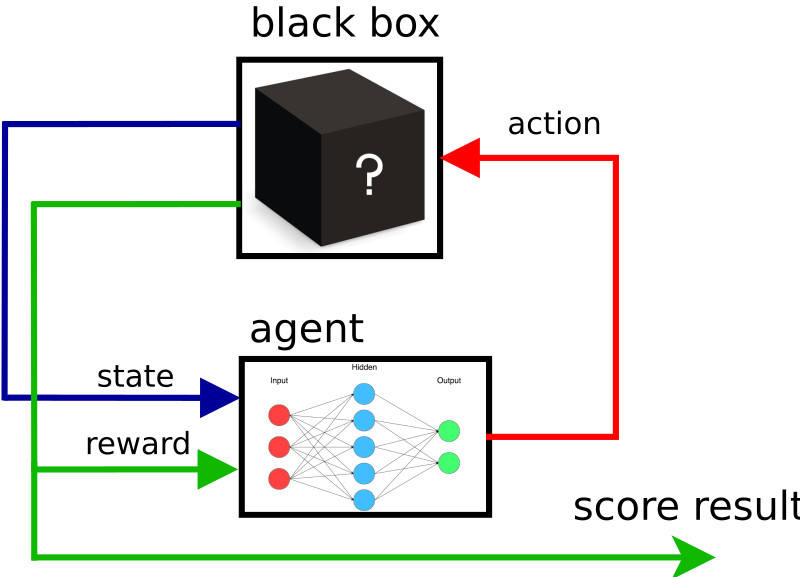
\includegraphics[scale=0.27]{../diagrams/rl_mechanism.jpg}
\end{figure}

\begin {itemize}
  \item input : state, reward
  \item output: action
\end{itemize}

\end{frame}


\begin{frame}{\bf SARSA algorithm}
State Action Reward State Action \footnotemark
\begin{align*}
Q'(s, a) = (1-\alpha)Q(s, a) + \alpha(R(s, a) + \gamma Q(s', a'))
\end{align*}
where \\
$Q(s, a)$ is previous state \\
$Q(s', a')$ is actual state \\
$R(s, a)$ is reward obtained in state $s$ after executing action $a$ \\
$\gamma$ is discount factor $\gamma \in \langle0, 1\rangle$ \\
$\alpha$ is learning rate $\alpha \in (0, 1)$
\begin{figure}[htbp]
  \centering
  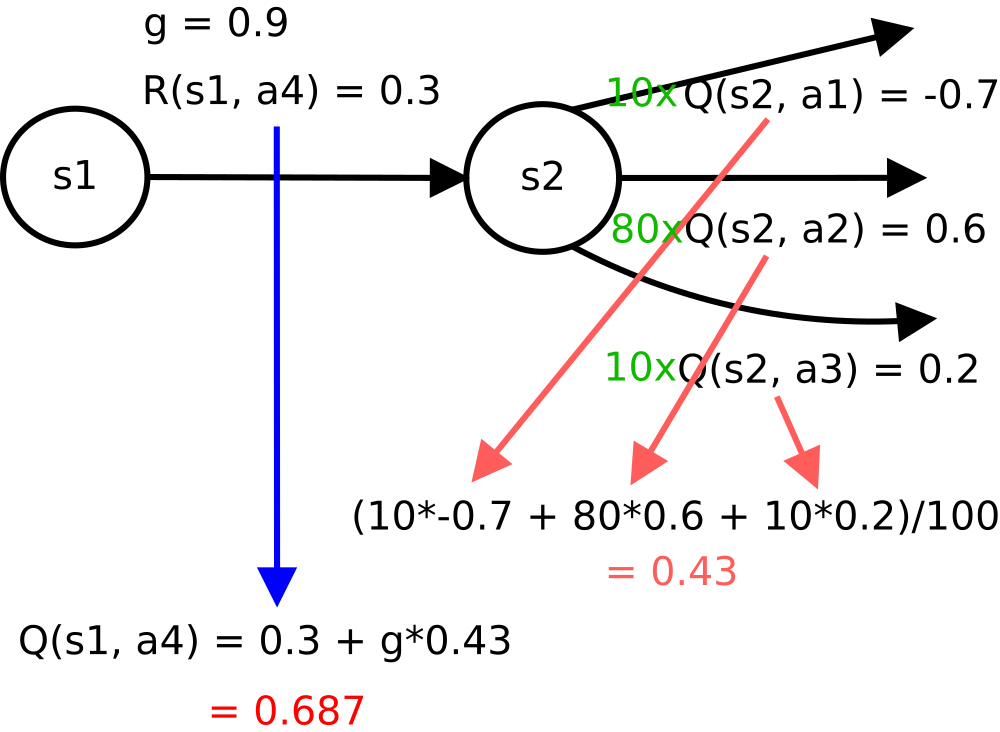
\includegraphics[scale=0.13]{../diagrams/sarsa_learning_detail.png}
\end{figure}

\footnotetext[1]{\tiny{Online Q-Learning using Connectionist Systems, by Rummery \& Niranjan (1994)}}


\end{frame}

\begin{frame}{\bf SARSA algorithm is recurrent}

Main learning mechanism : \\
learn previous $Q(s, a)$ from actual $Q(s', a')$. \\

\begin{figure}[htbp]
  \centering
  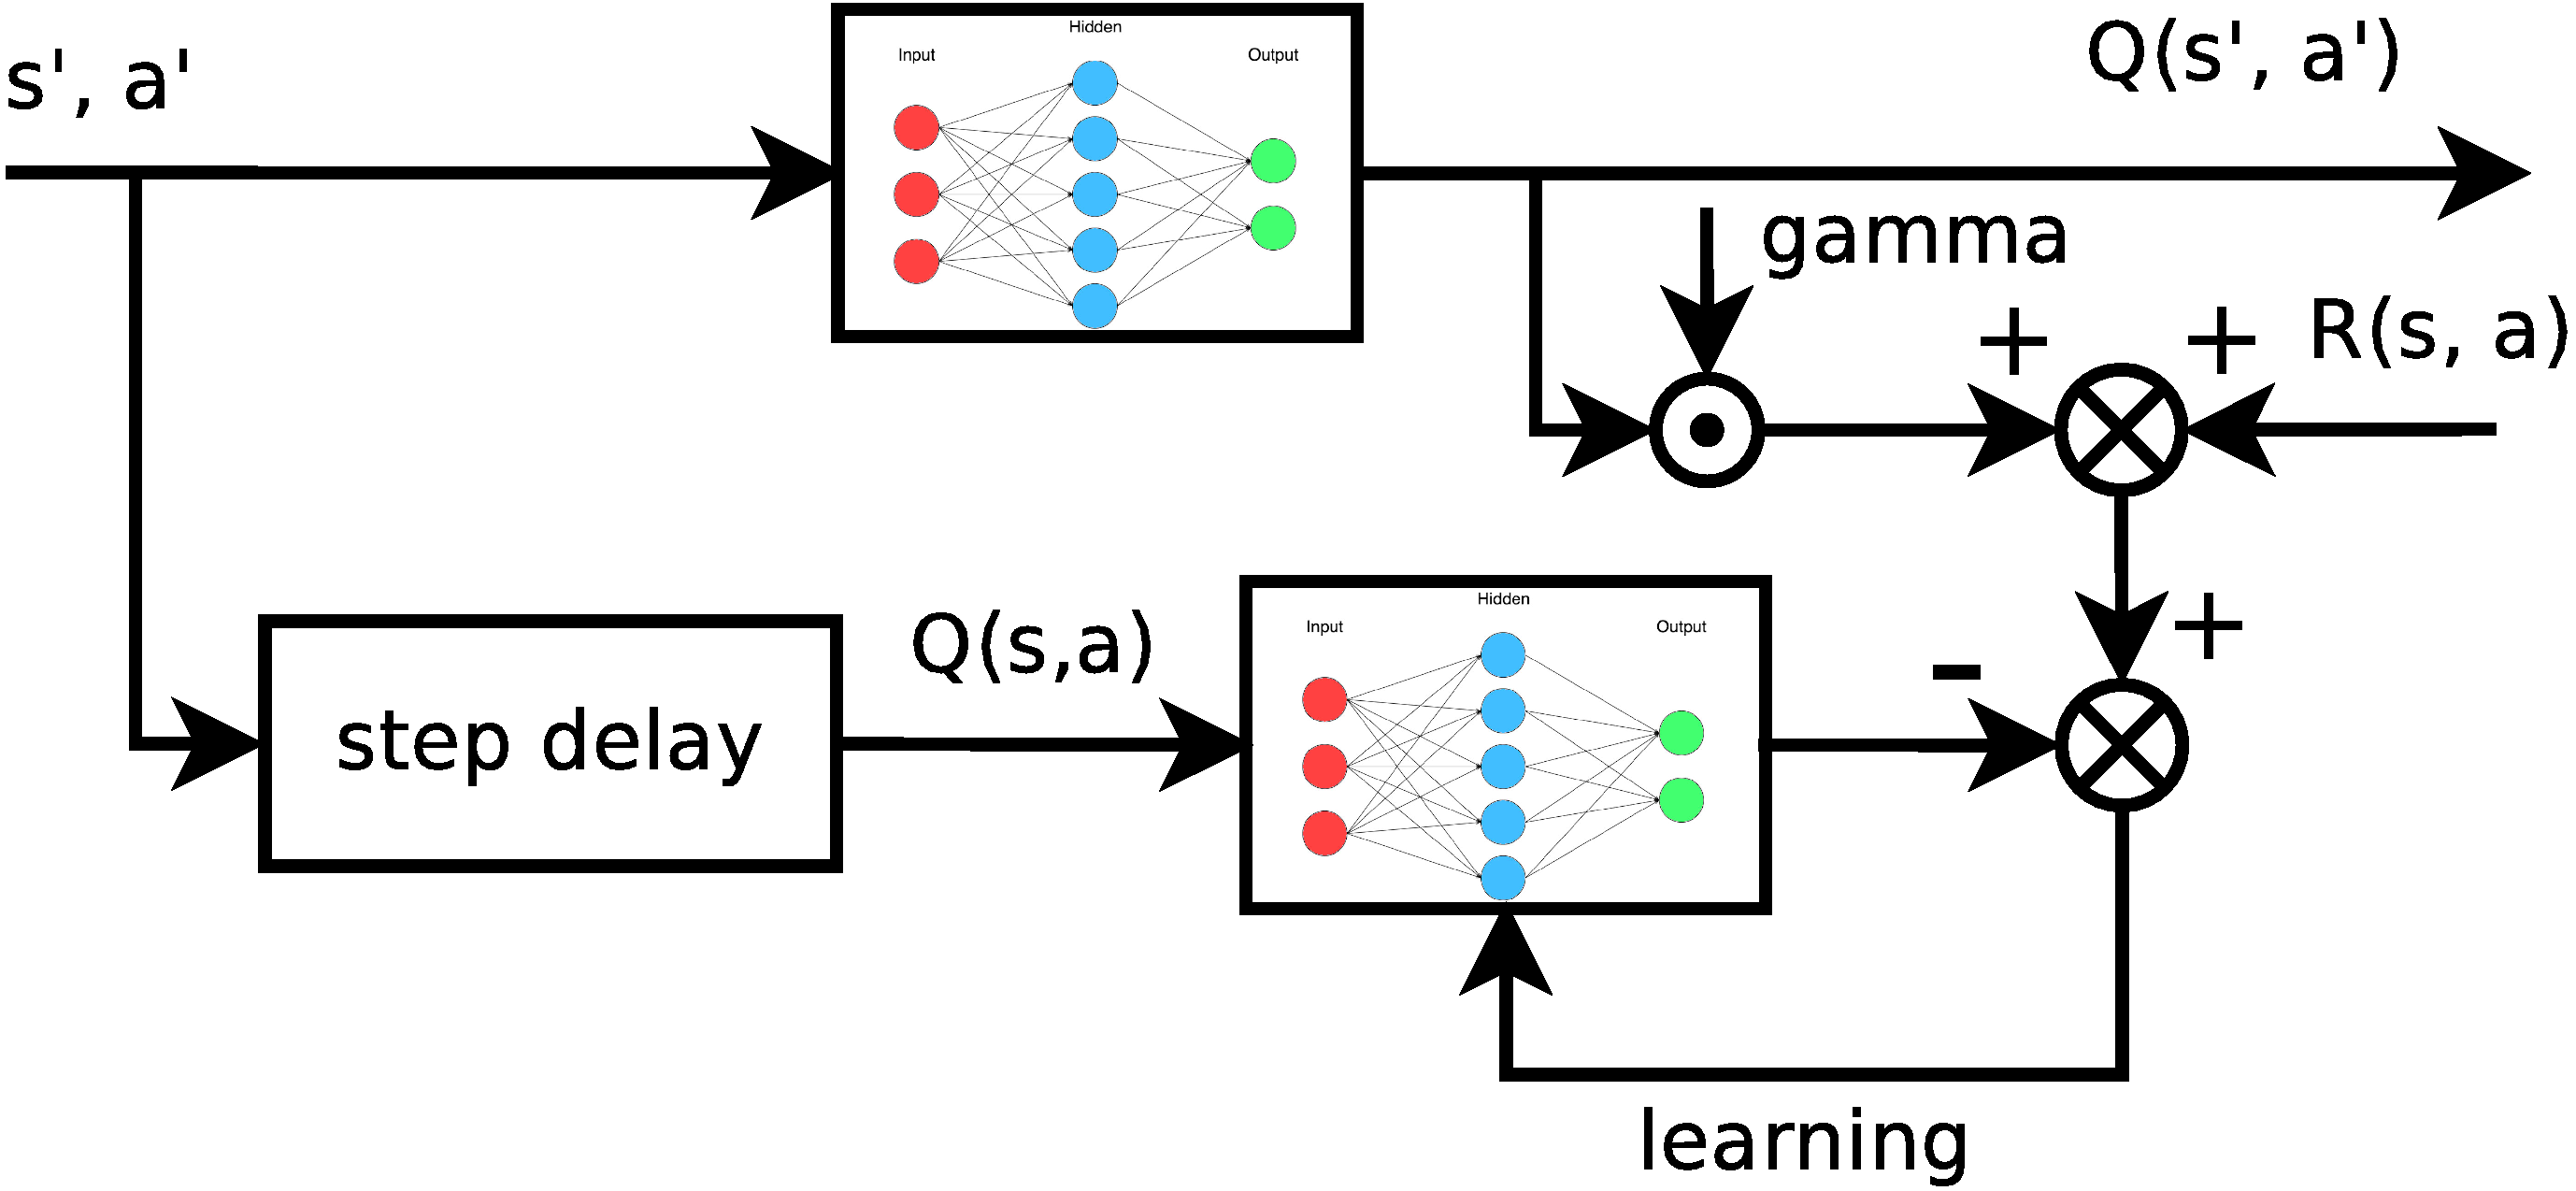
\includegraphics[scale=0.4]{../diagrams/rl_recurrent.png}
\end{figure}

\end{frame}


\begin{frame}{\bf SARSA algorithm is recurrent}

Main learning mechanism : \\
learn previous $Q(s, a)$ from actual $Q(s', a')$. \\

\begin{align*}
Q(n+1) &= R(n+1) + \gamma Q(n+2) \\
{\color{red} Q(n)} &= R(n) + \gamma Q(n+1) \\
{\color{blue} Q(n - 1)}&{\color{blue} = R(n-1) + \gamma }{\color{red} Q(n)} \text{// previous slide \footnotemark}\\
Q(n - 2) &= R(n-2) + \gamma Q(n-1)
\end{align*}

\begin{figure}[htbp]
  \centering
  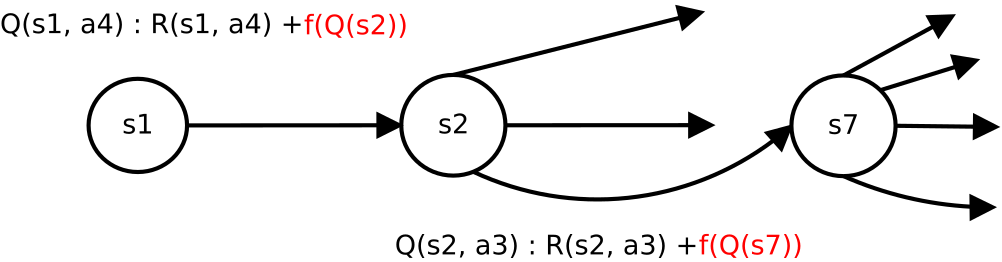
\includegraphics[scale=0.28]{../diagrams/sarsa_learning_detail_2.png}
\end{figure}

\footnotetext[1]{\tiny{equations are simplified, without $s$ and $a$}}



\end{frame}





\begin{frame}{\bf Q value approximation}

\begin{figure}[htbp]
  \centering
    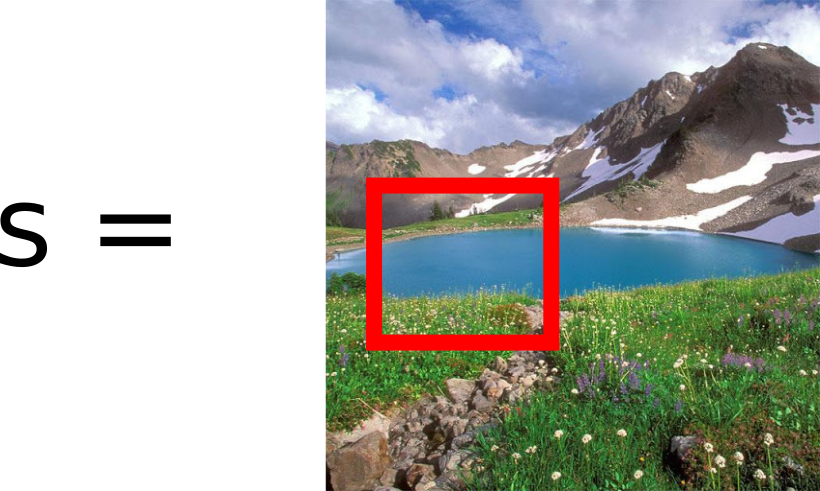
\includegraphics[scale=0.15]{../pictures/state_space.png}
\end{figure}

\begin{itemize}
  \item table
  \item linear combination of features
  \item neural network
  \item \bf{sparse representation}
\end{itemize}

\begin{figure}[htbp]
  \centering
    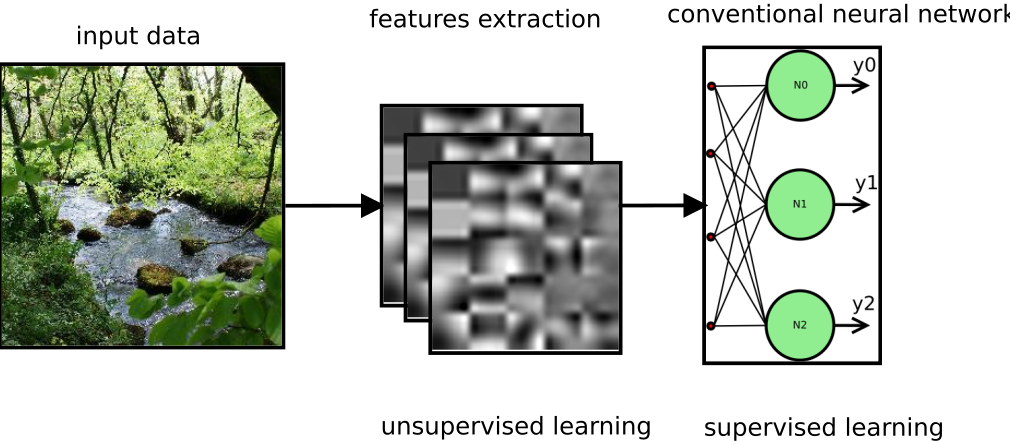
\includegraphics[scale=0.27]{../diagrams/features_nn.png}
\end{figure}


\end{frame}


\begin{frame}{\bf Q value approximation}
\Wider[4em]
{
Linear combination of $K$ {\bf learned} features $f_k(s)$, vector $v$ should be {\bf sparse}, why ?

\begin{flalign*}
&F(s) = \sum_{k=0}^{K-1} v_kf_k(s)&
\end{flalign*}

\begin{figure}
   \vspace{-80pt}%
   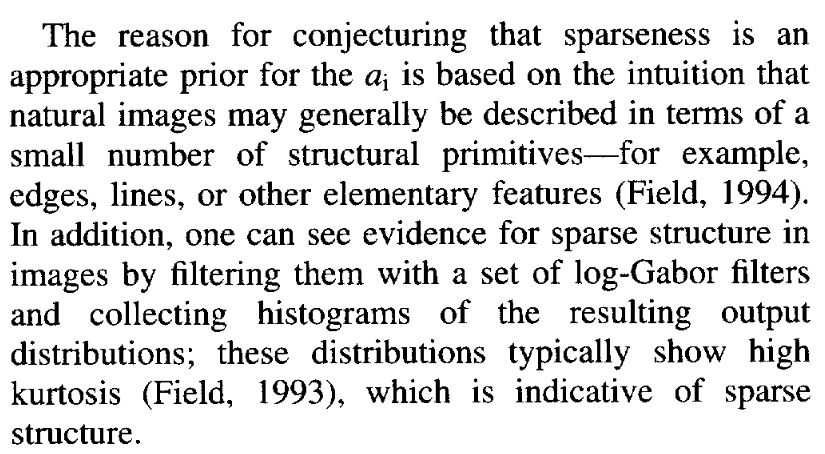
\includegraphics[scale=0.15, right]{../pictures/why_sparse.png}
   %\vspace{200pt}%
\end{figure}
}

\footnotetext[1]{\tiny{Olshausen and Field (1997): Sparse coding with an overcomplete basis set}}
\footnotetext[2]{\tiny{Olshausen BA, Field DJ (2004) : Sparse coding of sensory inputs. Current Opinion in Neurobiology, 14, 481-487}}
\footnotetext[3]{\tiny{Mushroom body, locust  (Laurent)}}
\footnotetext[4]{\tiny{HVC, zebra finch (Fee)}}
\footnotetext[5]{\tiny{Auditory cortex, mouse  (DeWeese \& Zador)}}
\footnotetext[6]{\tiny{Hippocampus, rat\/primate(Thompson \& Best; Skaggs)}}
\footnotetext[7]{\tiny{Motor cortex, rabbit  (Swadlow)}}
\footnotetext[8]{\tiny{Visual cortex, monkey\/cat  (Vinje \& Gallant)}}
\footnotetext[9]{\tiny{Inferotemporal cortex, human (Fried \& Koch)}}


\end{frame}


\begin{frame}{\bf Looking for symmetry}

\begin{itemize}
\item Euler-Lagrange equation
\item Noether's theorem
\item Conservation law
\end{itemize}

\Wider[4em]
{
\begin{flalign*}
S(q) = \int_{a}^{b}L \Big( t, q(t), \frac{dq(t)}{dt} \Big)  dt
\end{flalign*}

\begin{figure}
   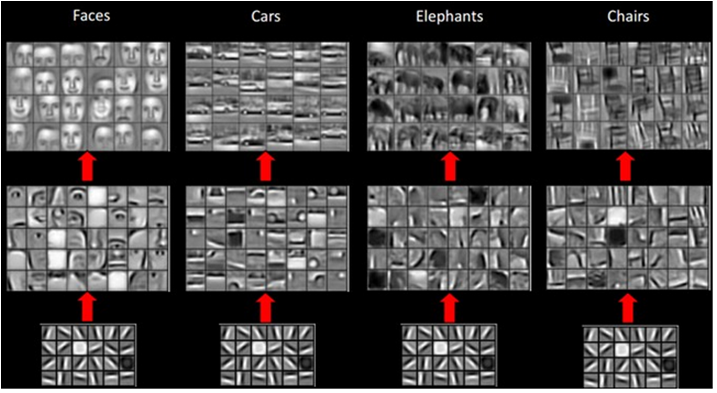
\includegraphics[scale=1.3, center]{../pictures/deep_nn_features.png}
\end{figure}
}

\end{frame}



\begin{frame}{\bf Sparse representation}
\Wider[4em]
{
\begin{flalign*}
F(s) = \sum_{k=0}^{K-1} v_kf_k(s)
\end{flalign*}

\begin{figure}
   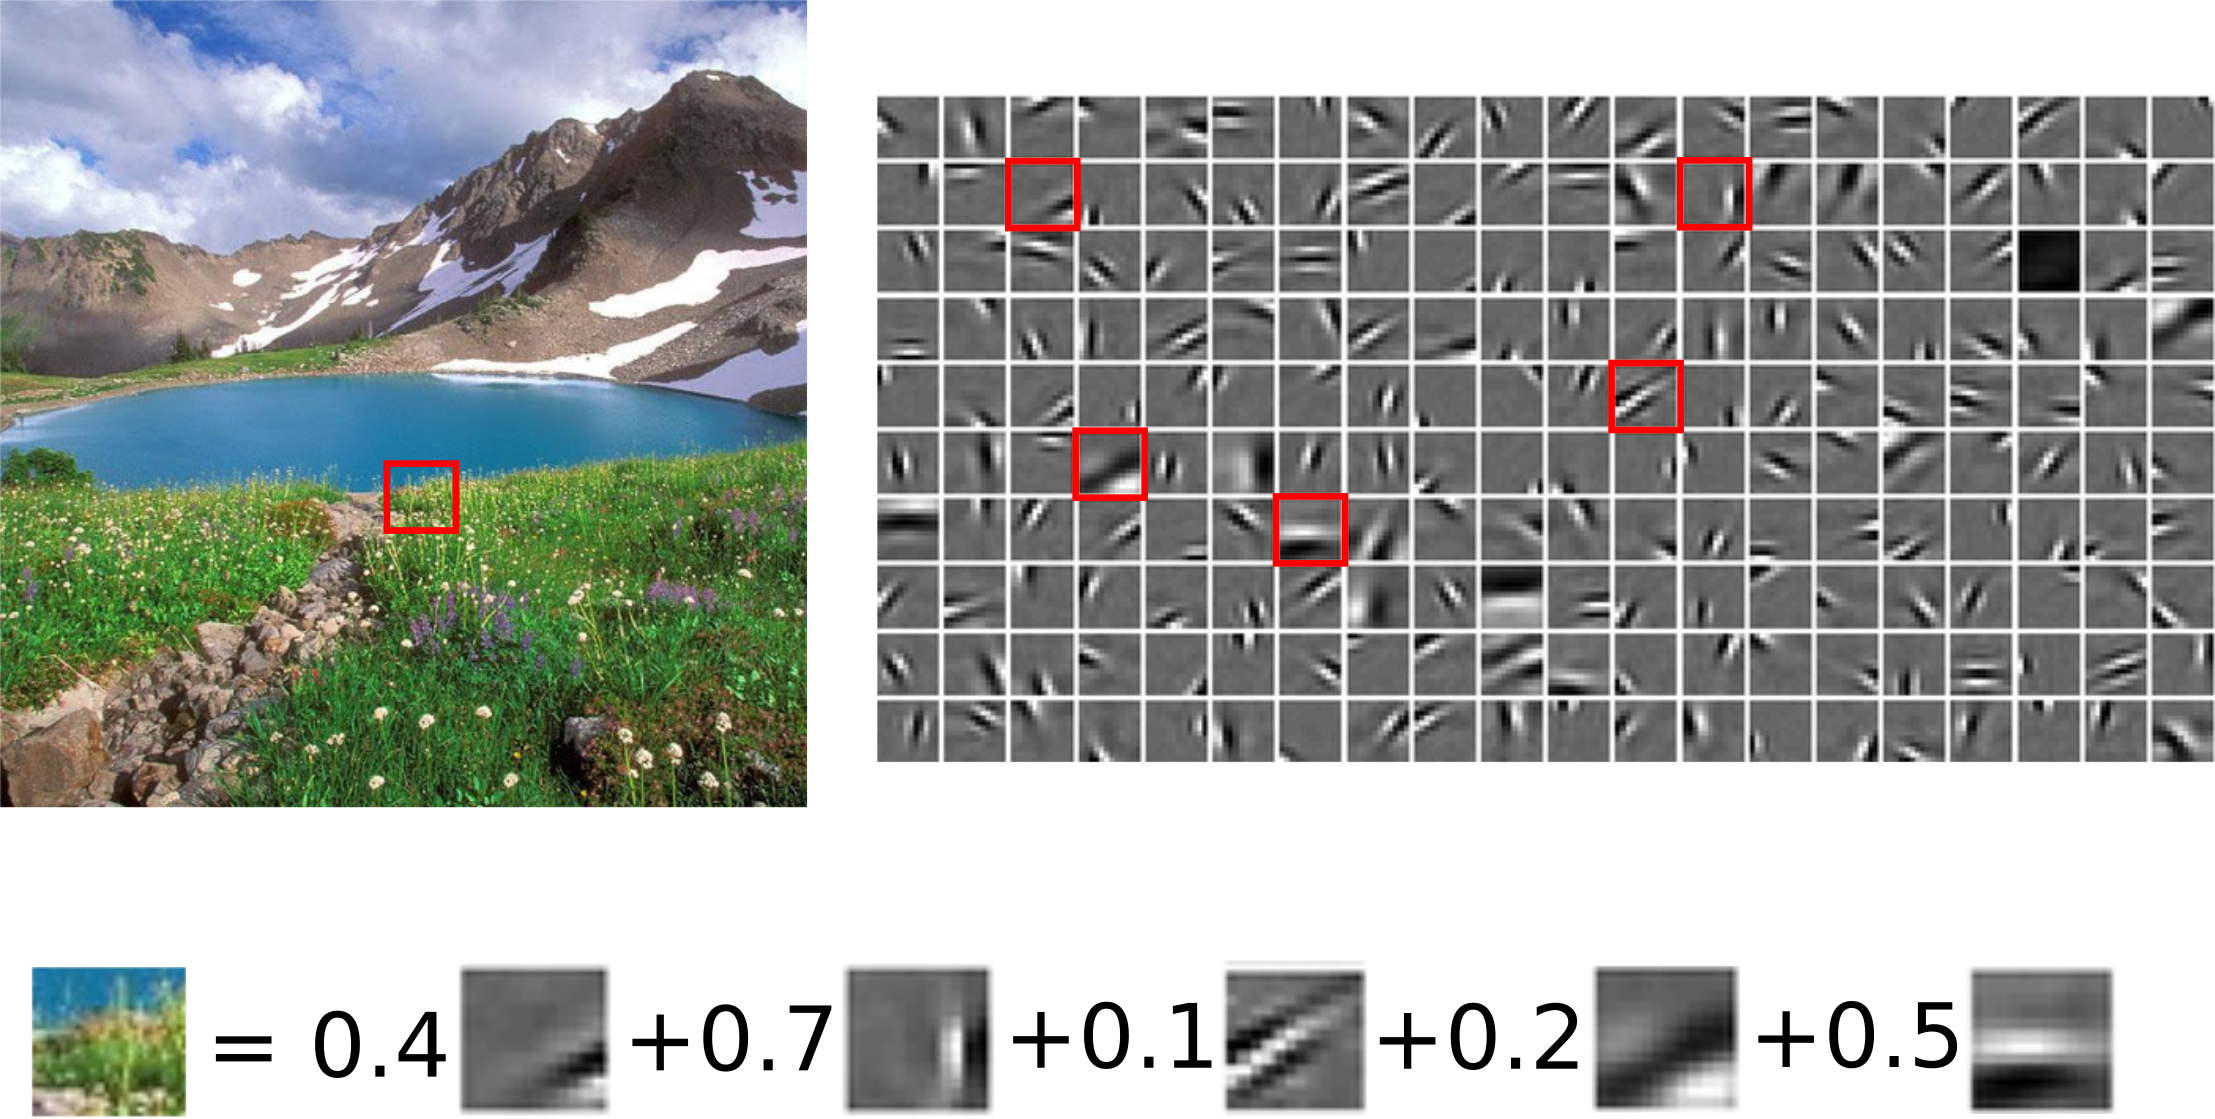
\includegraphics[scale=0.3, center]{../diagrams/sparse_dictionary.png}
\end{figure}
}

\end{frame}




\begin{frame}{\bf Sparse representation}

\begin{align*}
E(w, y) &= \sum_{k=0}^{K-1} \left\Vert x_k - wy_k \right\Vert^2_2 + \lambda_0 \left\Vert y_k \right\Vert^2_1 + \lambda_1 \left\Vert w \right\Vert^2_{2,1} \\
&\text{subject to} \quad y_{ki} > 0
\end{align*}

\begin{itemize}
  \item
      reconstruction condition
      \begin{align*}
      \left\Vert x_k - wy_k \right\Vert^2_2
      \end{align*}
      \color{black}


  \item
      $y_k$ sparsity condition
      \begin{align*}
      \lambda_0 \left\Vert y_k \right\Vert^2_1
      \end{align*}


  \item
      $w$ sparsity condition
      \begin{align*}
      \lambda_1 \left\Vert w \right\Vert^2_{2,1}
      \end{align*}
\end{itemize}

\end{frame}


\begin{frame}{\bf Estimating $W$ and $Y$ - modified K-SVD algorithm}

\begin{algorithm}[H]
 \KwData{W, depth, X}
 \KwResult{sparse representation Y, features matrix weights W }
 initialization  \\
                $W \gets random$, $R \gets X$ \\
                $\eta$ learning rate, $\epsilon$ shrink value \\
 \For{j from 0 to depth}
 {
  \color{blue}
  $best = \arg\max\limits_{i} W[i] R $ \\
  \color{red}
  $d = ReLU (\frac{W[best] R}{\Vert W[best]\Vert^2_2})$ \\
  $Y[best] = d$ \\
  \color{black}
  \For{i from 0 to size(R)}
  {
    $dw = d(R[i] - W[best][i])$ \\
    $W[best][i] = W[best][i] + \eta dw$ \\

    $W[best][i] = shrink(W[best][i], \epsilon)$

    \color{green}
    R[i] = R[i] - d*W[best][i]
  }
 }
\end{algorithm}

\begin{figure}
   \vspace{-210pt}%
   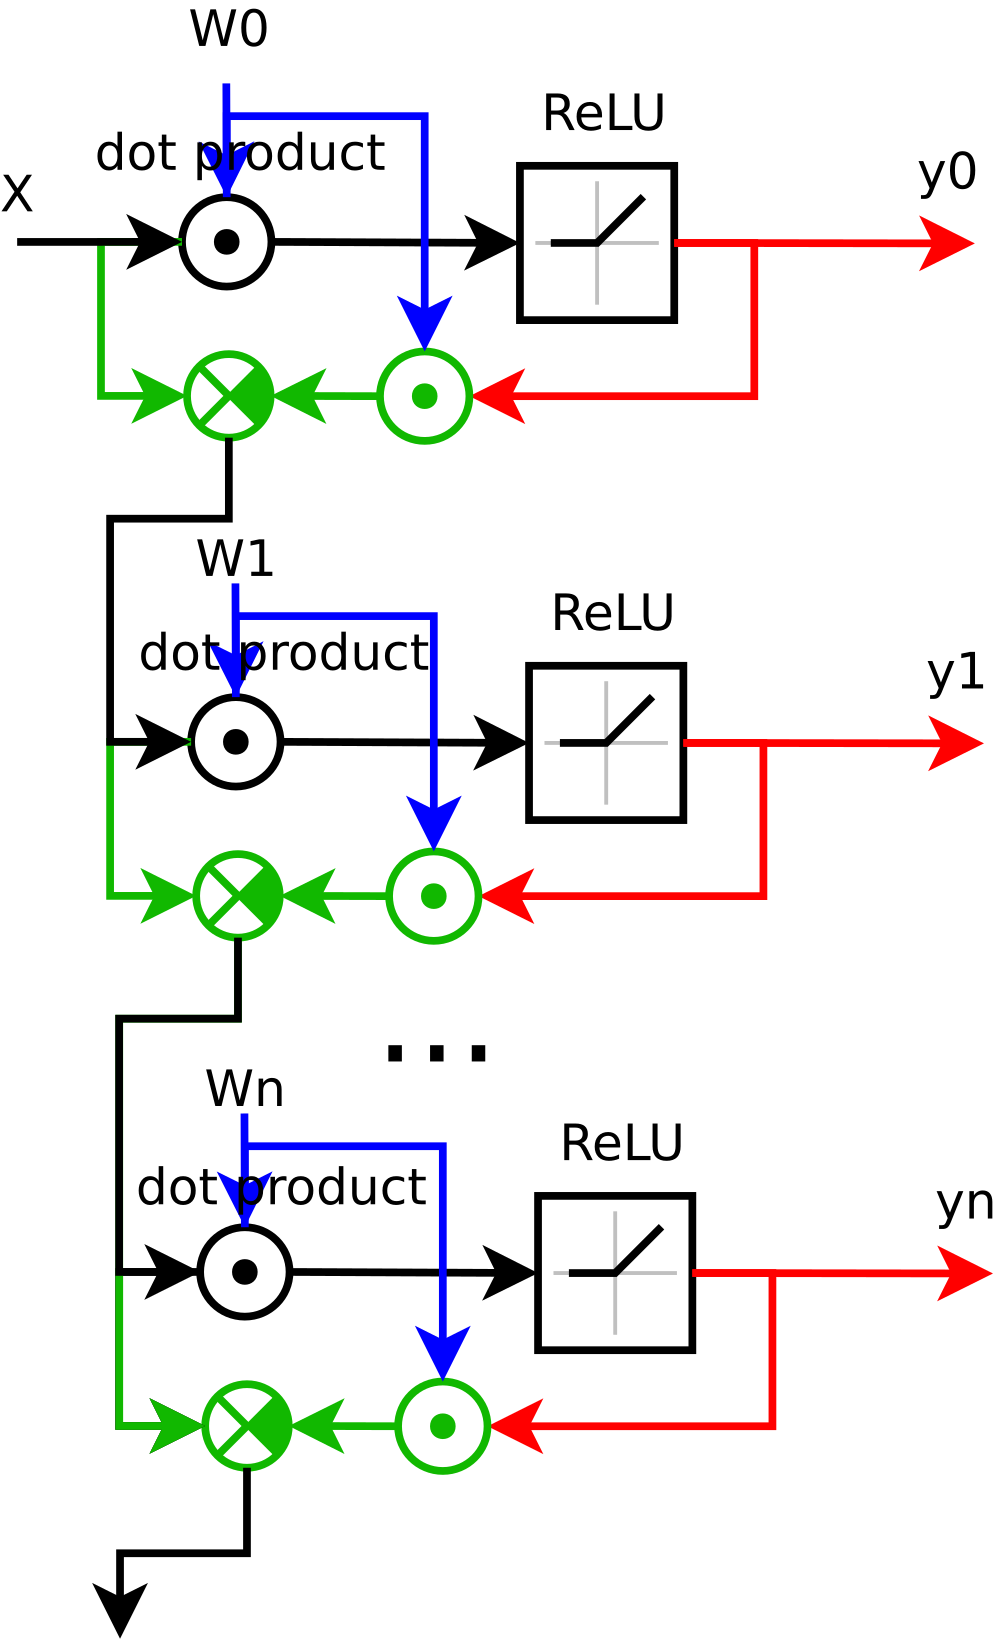
\includegraphics[scale=0.13, right]{../diagrams/features_layer_01.png}
\end{figure}

\end{frame}


\begin{frame}{\bf Advanced sparse distributed memory}

\centering

\begin{figure}[C]
   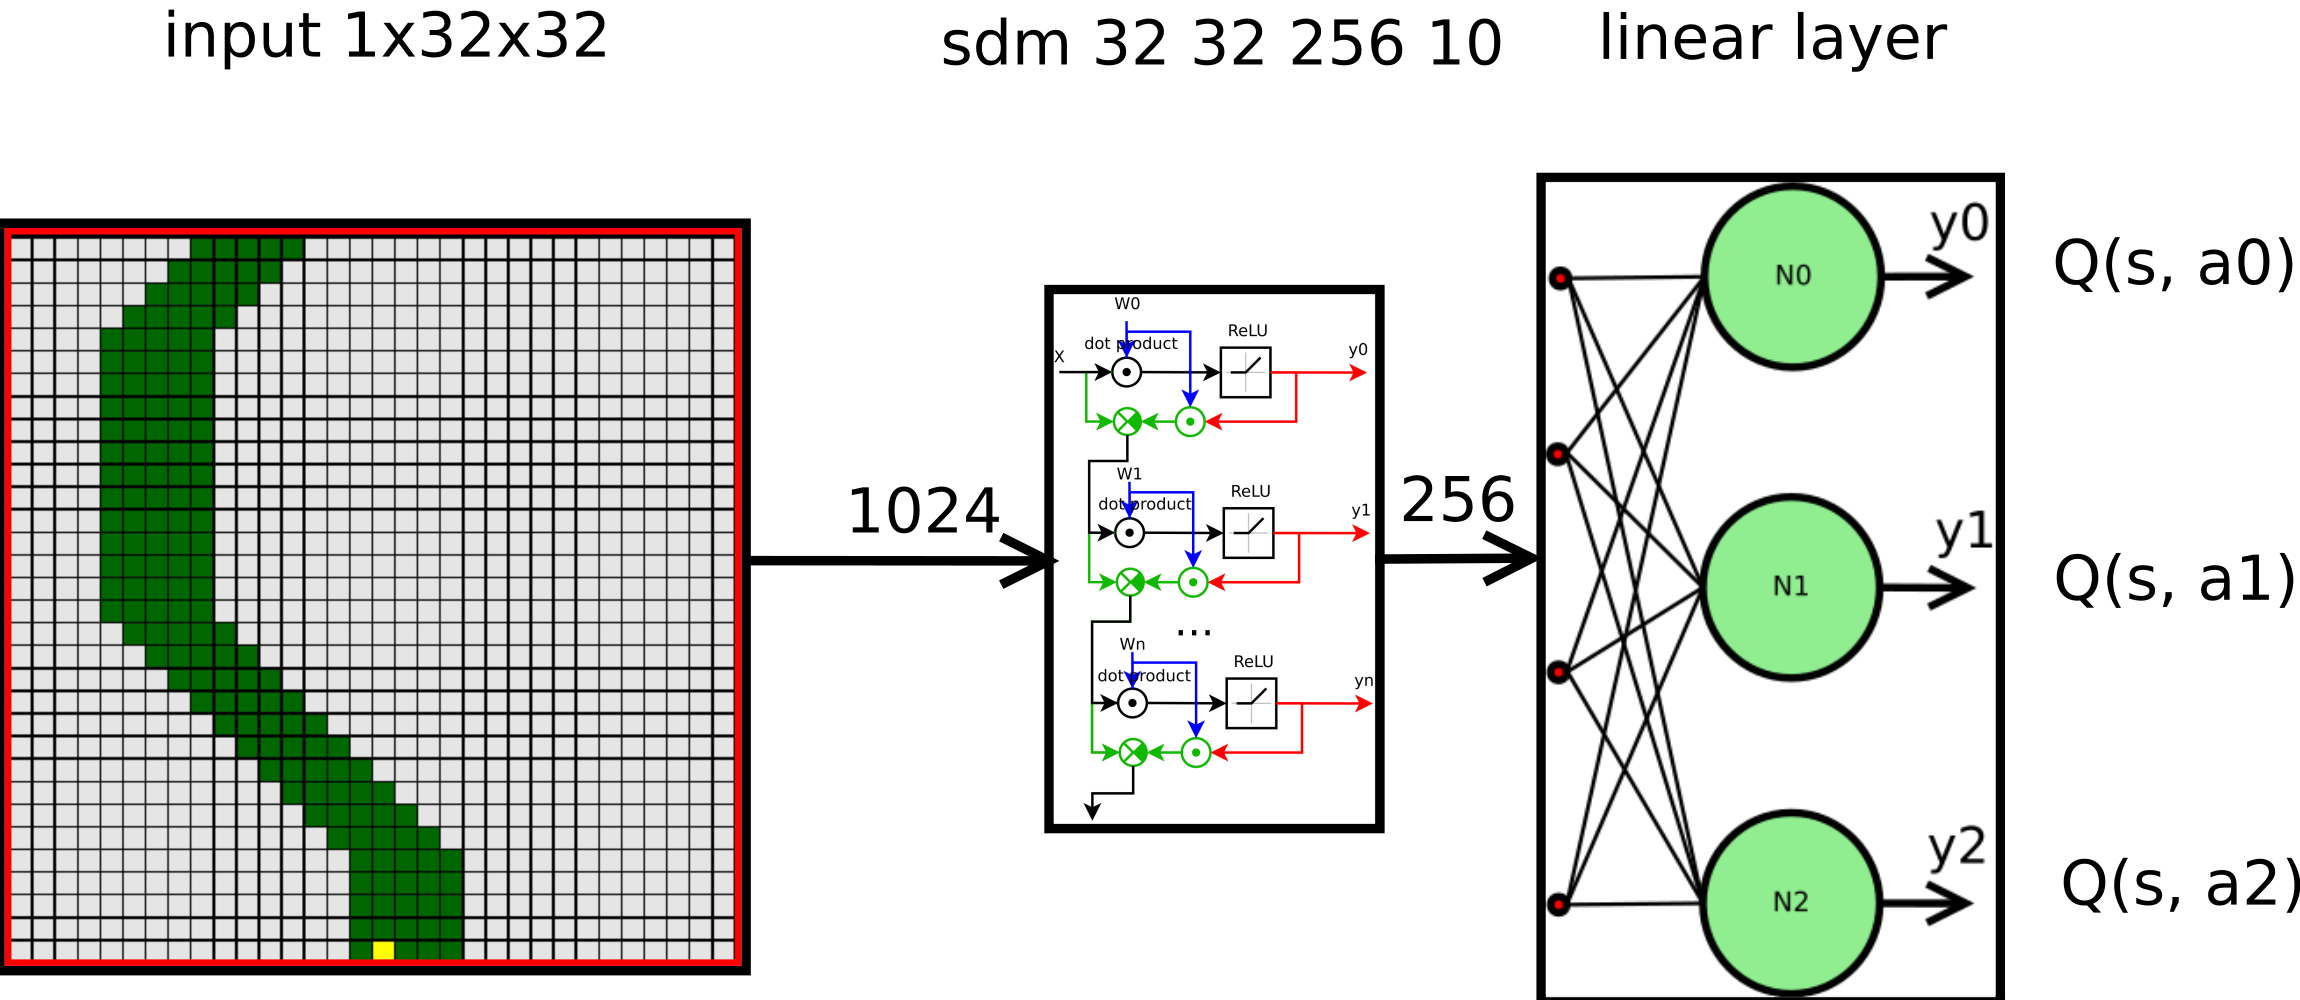
\includegraphics[scale=0.18]{../diagrams/convolution_01.png}
\end{figure}

\end{frame}


\begin{frame}{\bf Advanced sparse distributed memory + Convolution}

\centering

\begin{figure}[C]
   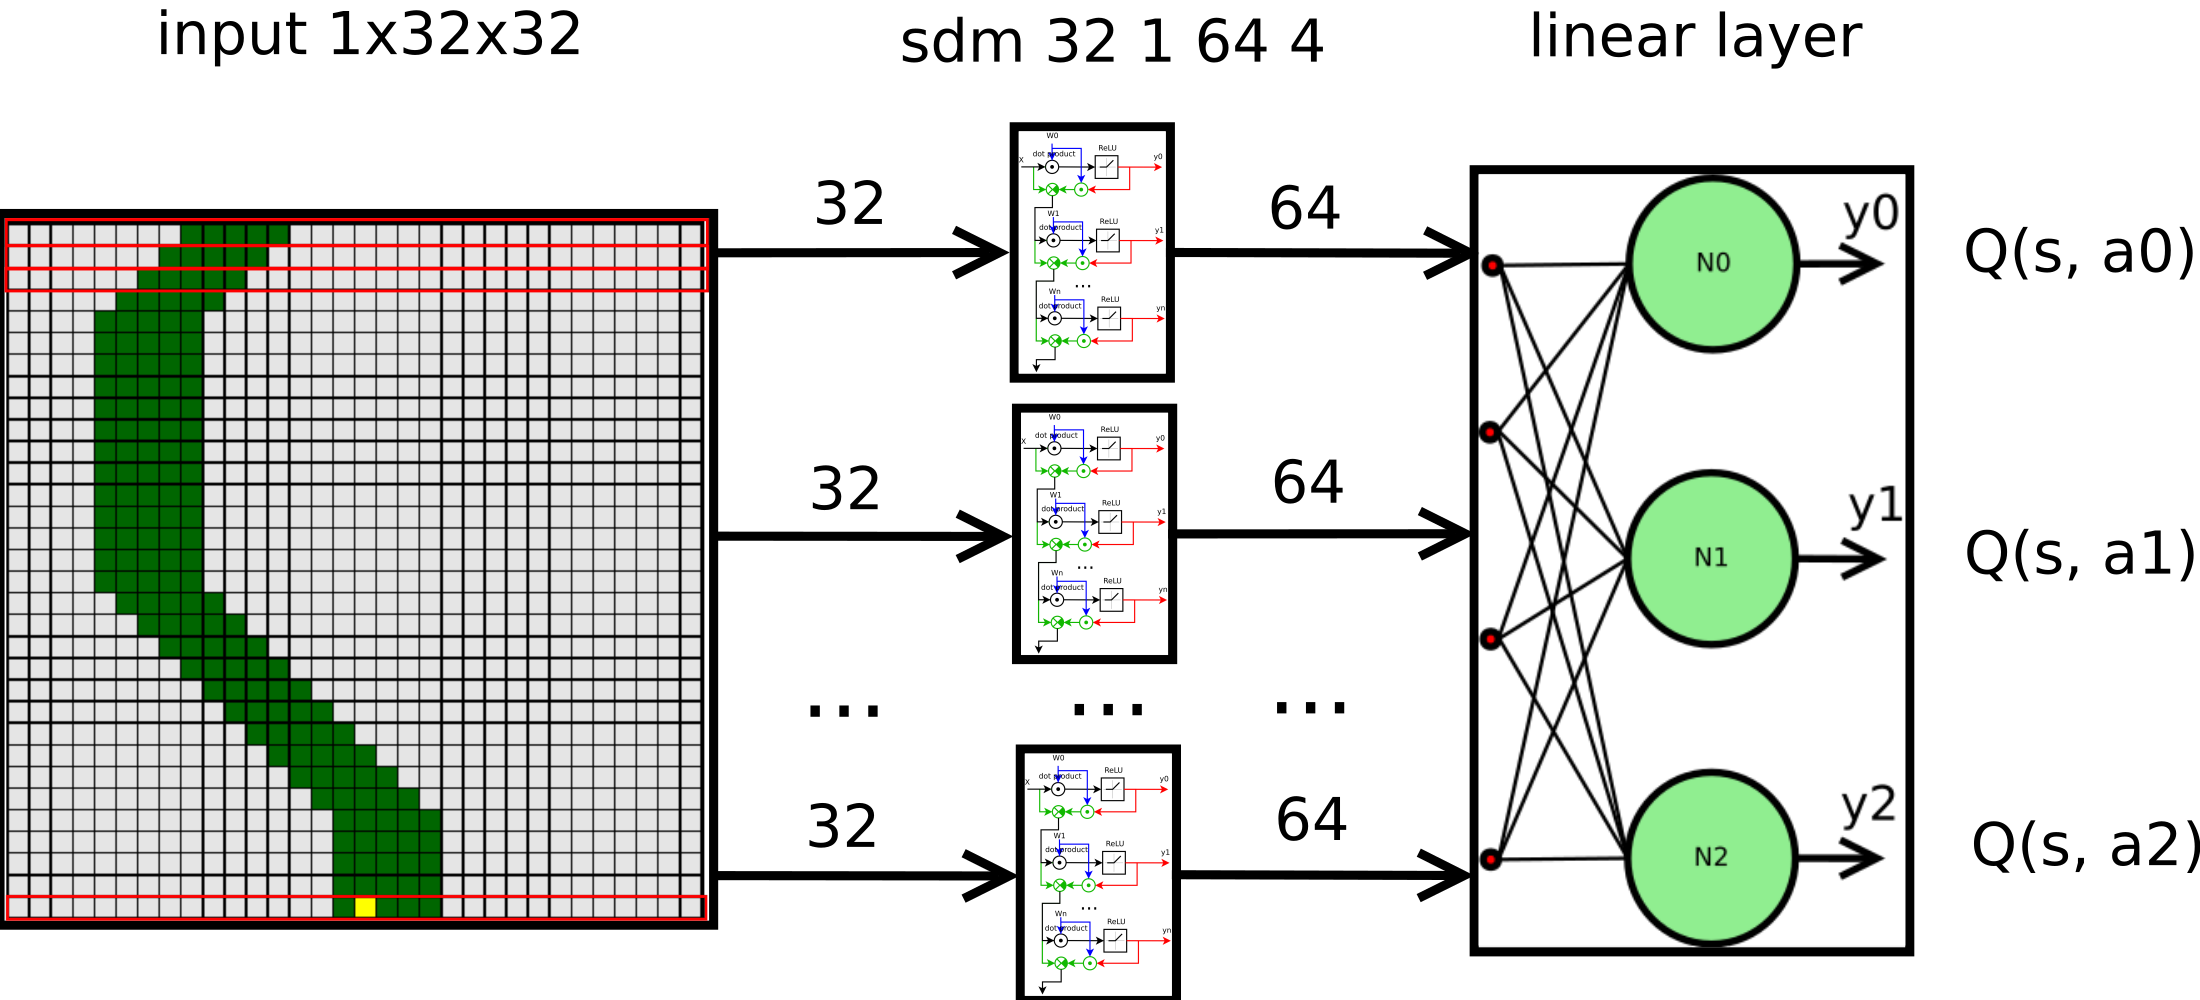
\includegraphics[scale=0.18]{../diagrams/convolution_02.png}
\end{figure}

\end{frame}


\begin{frame}{\bf  Advanced sparse distributed memory + Convolution + Deep layer}

\centering

\begin{figure}[C]
   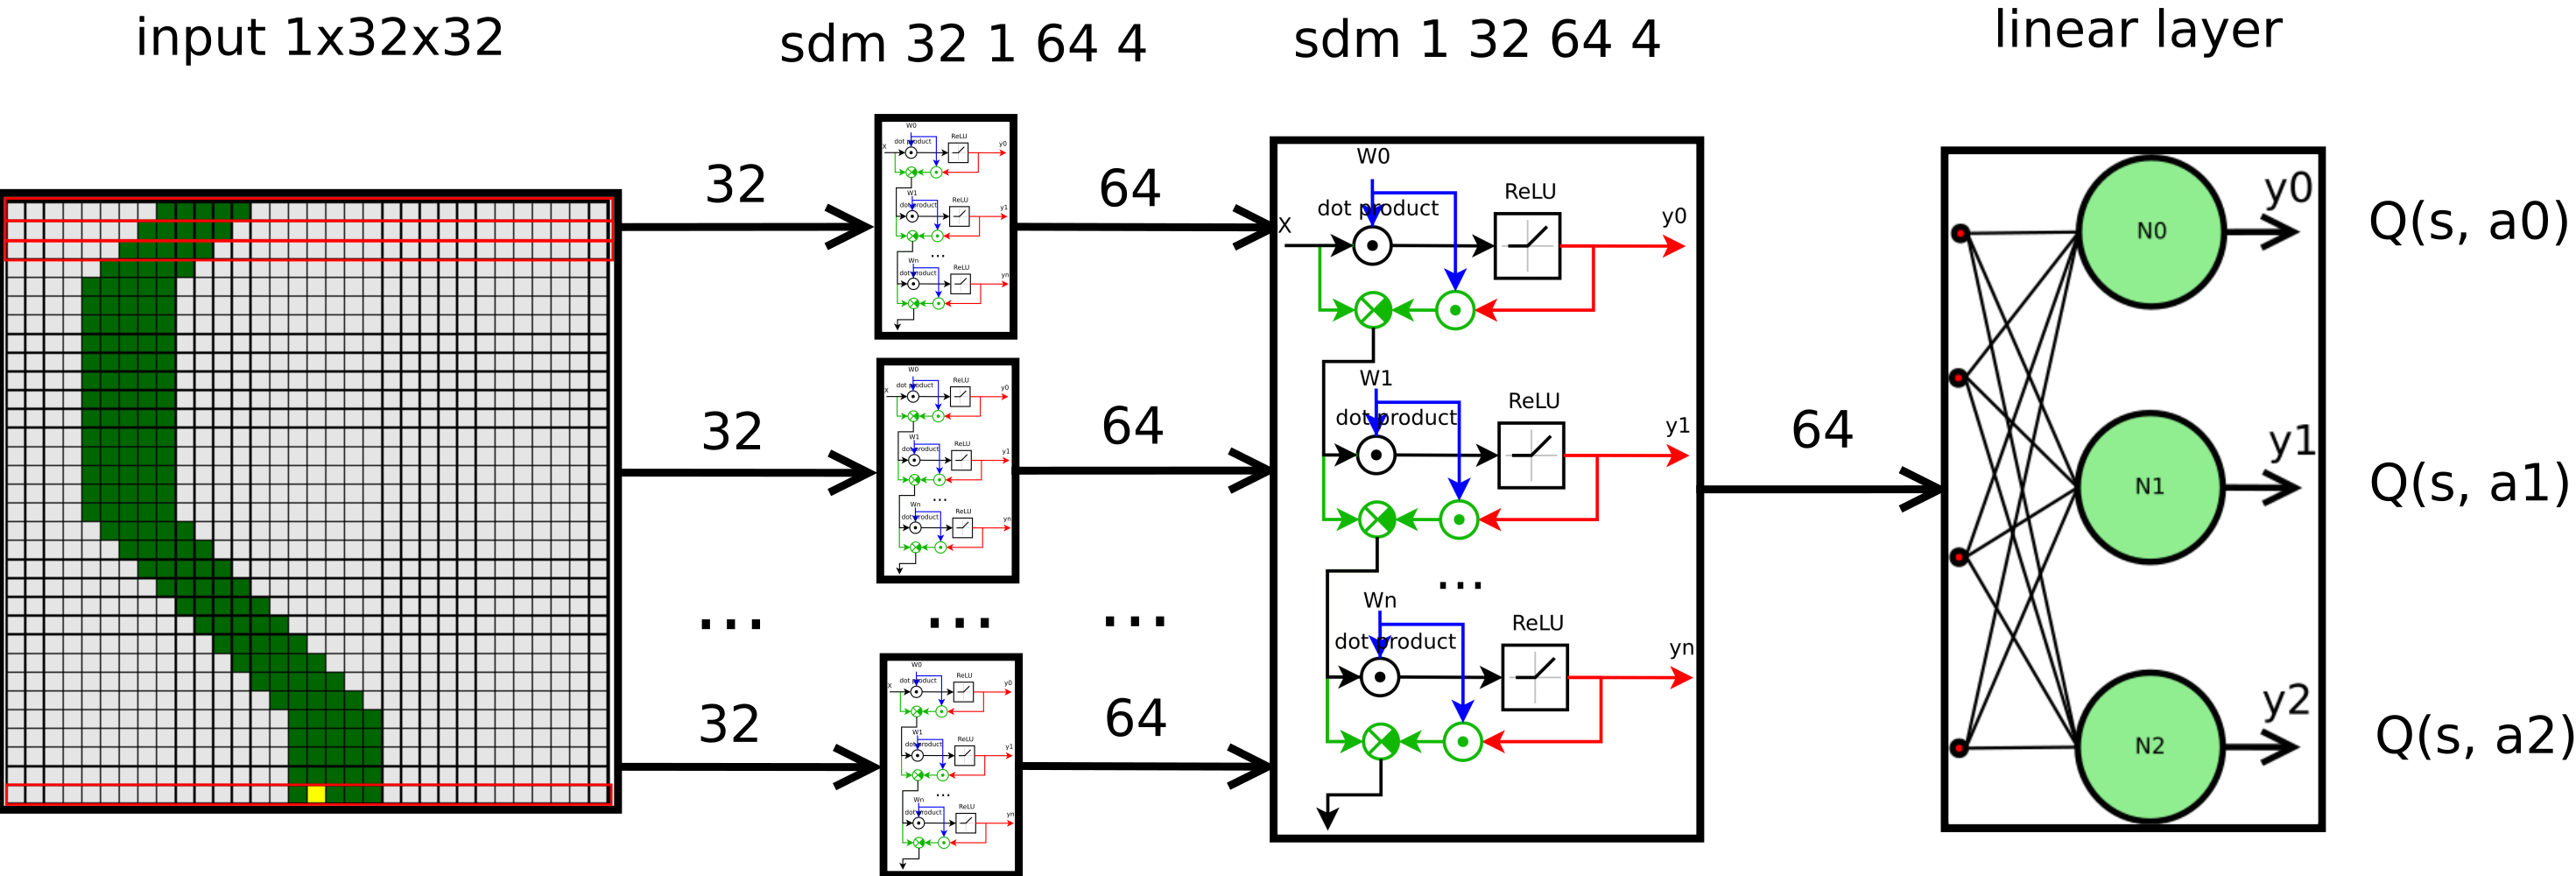
\includegraphics[scale=0.14]{../diagrams/convolution_03.png}
\end{figure}

\end{frame}

\begin{frame}{\bf Experimental results}

\begin{itemize}
  \item Mouse and food
  \item Worms
  \item Line follower
\end{itemize}

\end{frame}

\begin{frame}{\bf Mouse and food}

\begin{itemize}
  \item state : vector $64x\{0, 1\}$, 1 if mouse on field
  \item action : left, right, up, down
  \item reward : +1 for target hit, -1 for red hit
\end{itemize}

\begin{figure}[C]
   \includegraphics[scale=0.27]{../pictures/mouse_desc.png}
\end{figure}

\end{frame}

\begin{frame}{\bf Mouse and food}
\Wider[4em]
{

\begin{figure}
\centering
\begin{minipage}{.5\textwidth}
  \centering
  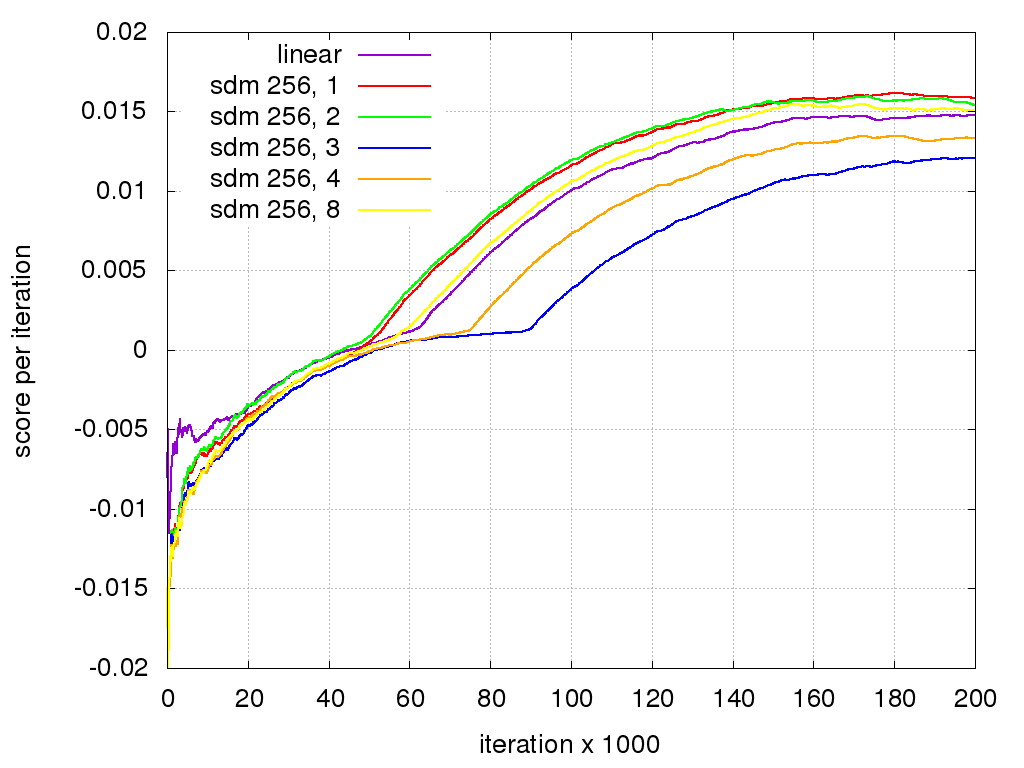
\includegraphics[width=1.0\linewidth]{{../results/mouse_result/progress_per_iteration_0.000}.png}
  \captionof*{figure}{Progress rate, state noise 0.0}
\end{minipage}%
\begin{minipage}{.5\textwidth}
  \centering
  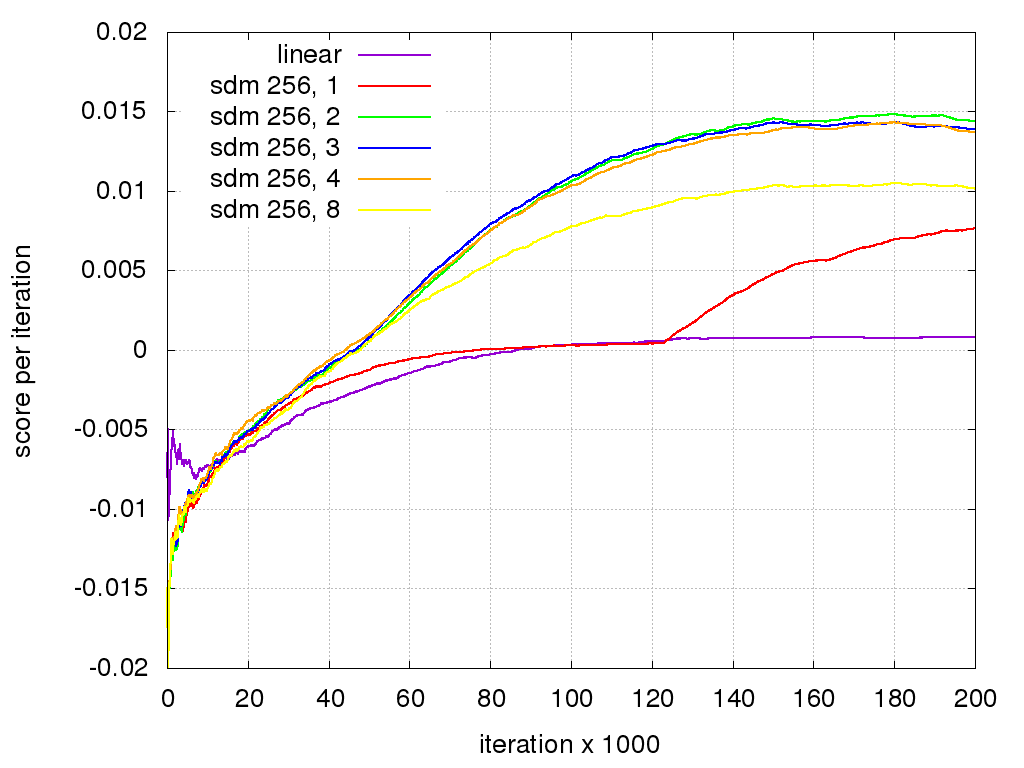
\includegraphics[width=1.0\linewidth]{{../results/mouse_result/progress_per_iteration_0.100}.png}
  \captionof*{figure}{Progress rate, state noise 0.1}
\end{minipage}
\end{figure}
}
\end{frame}



\begin{frame}{\bf Mouse and food - linear approximator}
\Wider[4em]
{

\begin{figure}
\centering
\begin{minipage}{.5\textwidth}
  \centering
  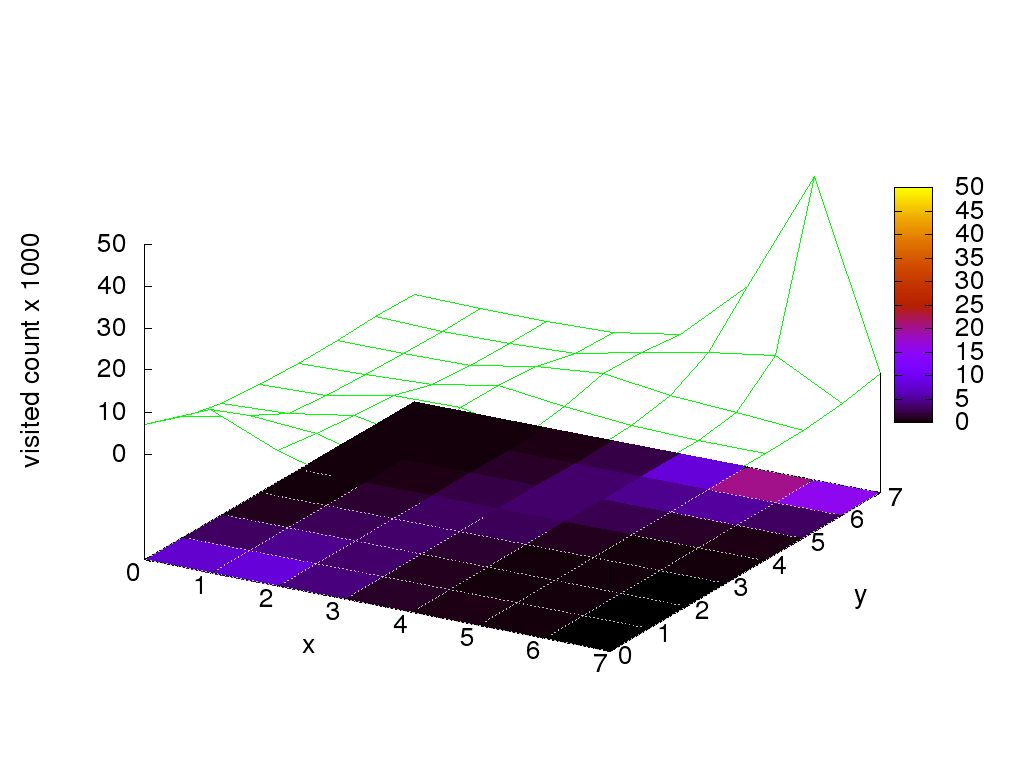
\includegraphics[width=1.0\linewidth]{{../results/mouse_result/linear_0.000__visited_fields}.png}
  \captionof*{figure}{Visited field rate, state noise 0.0}
\end{minipage}%
\begin{minipage}{.5\textwidth}
  \centering
  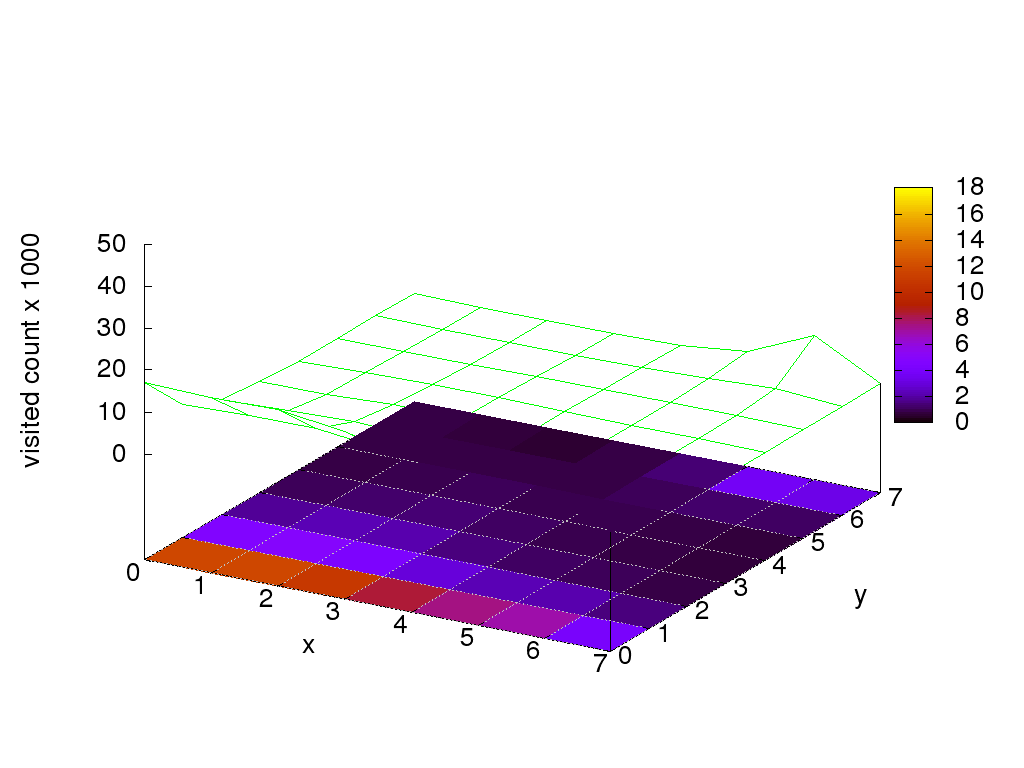
\includegraphics[width=1.0\linewidth]{{../results/mouse_result/linear_0.100__visited_fields}.png}
  \captionof*{figure}{Visited field rate, state noise 0.1}
\end{minipage}
\end{figure}
}
\end{frame}



\begin{frame}{\bf Mouse and food - sdm approximator 256, 2}
\Wider[4em]
{

\begin{figure}
\centering
\begin{minipage}{.5\textwidth}
  \centering
  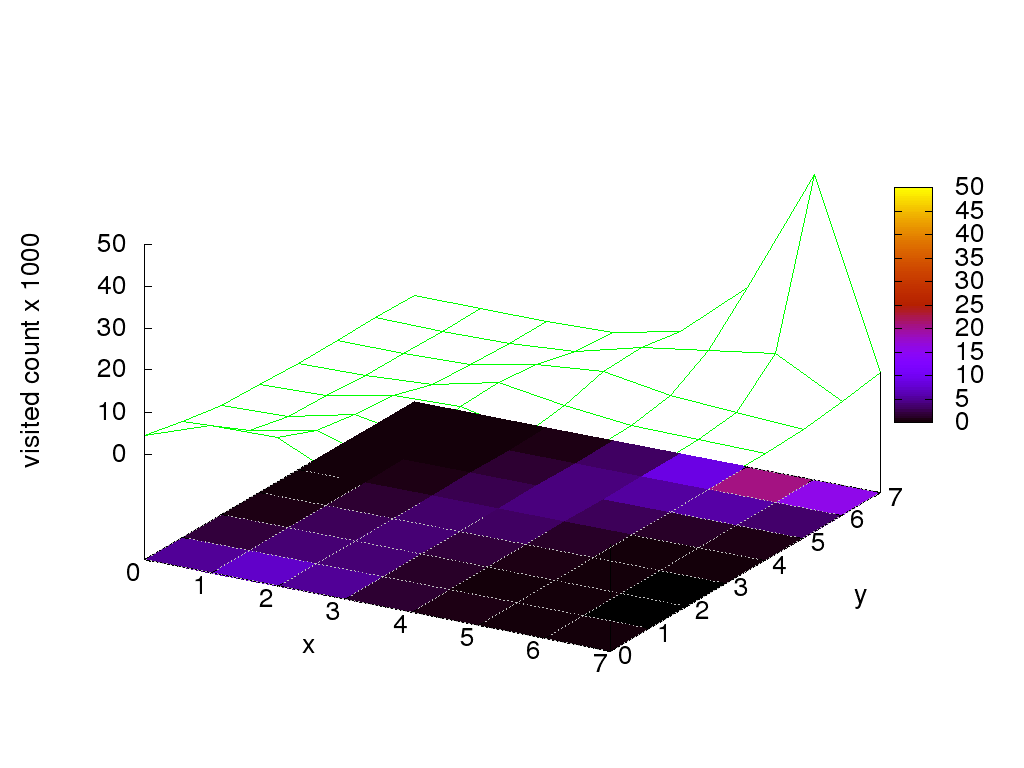
\includegraphics[width=1.0\linewidth]{{../results/mouse_result/sdm_0.000_256_2_visited_fields}.png}
  \captionof*{figure}{Visited field rate, state noise 0.0}
\end{minipage}%
\begin{minipage}{.5\textwidth}
  \centering
  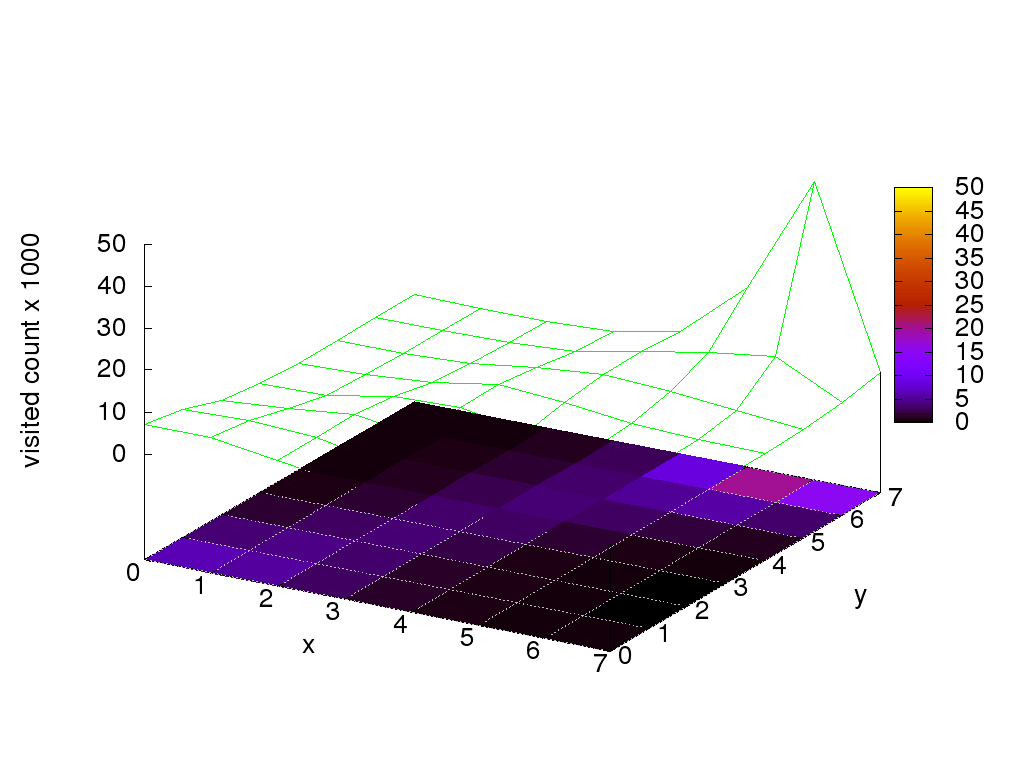
\includegraphics[width=1.0\linewidth]{{../results/mouse_result/sdm_0.100_256_2_visited_fields}.png}
  \captionof*{figure}{Visited field rate, state noise 0.1}
\end{minipage}
\end{figure}
}
\end{frame}


\begin{frame}{\bf Worms}

\centering
\begin{figure}[C]
   \includegraphics[scale=0.27]{../pictures/sdm_demo_desc.png}
\end{figure}

\end{frame}



\begin{frame}{\bf Worms - memory size and activity results}
\Wider[4em]
{

\begin{figure}
\centering
\begin{minipage}{.5\textwidth}
  \centering
  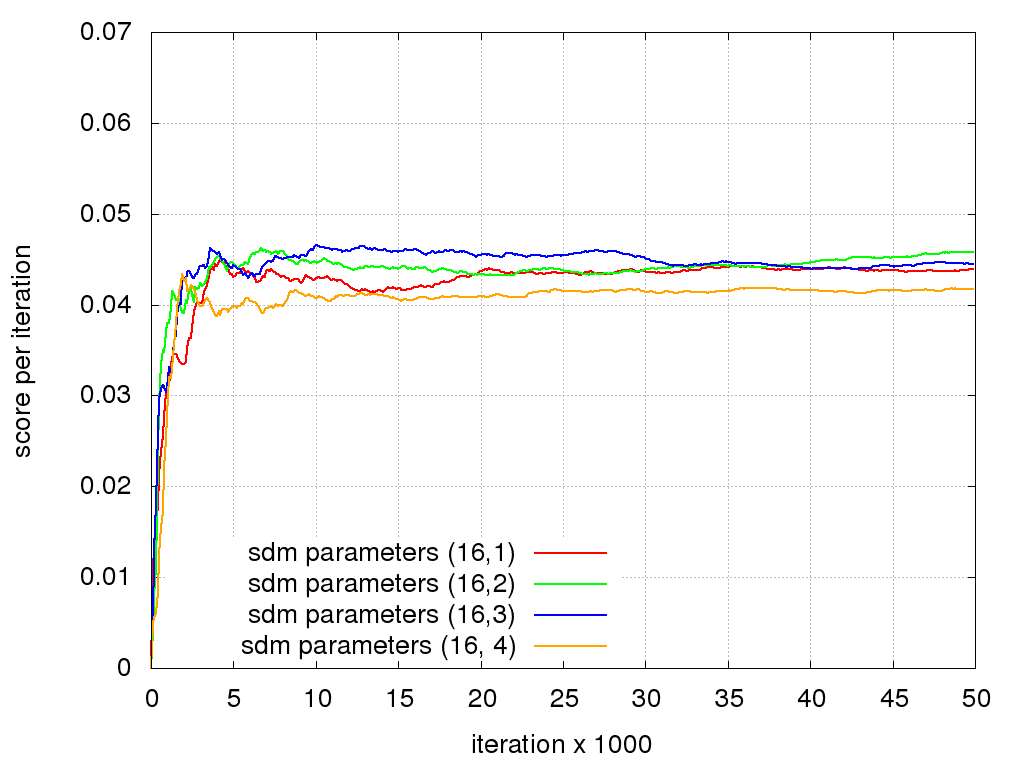
\includegraphics[width=1.0\linewidth]{{../results/worms_result/progress_experiment_/progress_per_iteration_16}.png}
\end{minipage}%
\begin{minipage}{.5\textwidth}
  \centering
  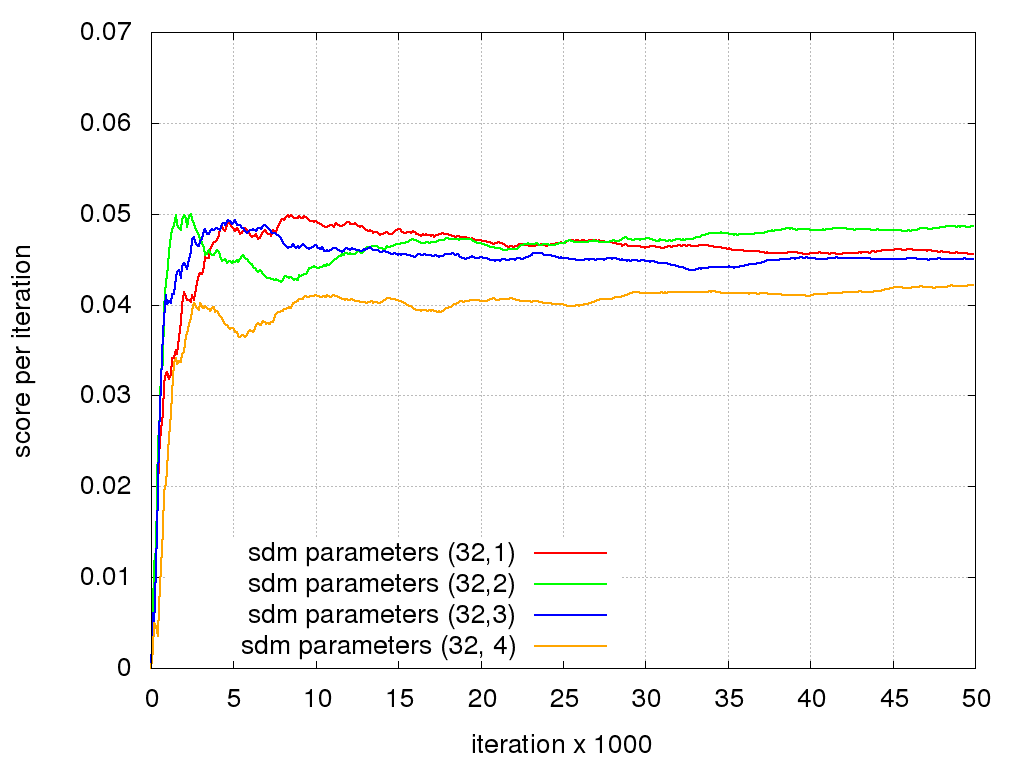
\includegraphics[width=1.0\linewidth]{{../results/worms_result/progress_experiment_/progress_per_iteration_32}.png}
\end{minipage}
\end{figure}
}
\end{frame}




\begin{frame}{\bf Worms - memory size and activity results}
\Wider[4em]
{

\begin{figure}
\centering
\begin{minipage}{.5\textwidth}
  \centering
  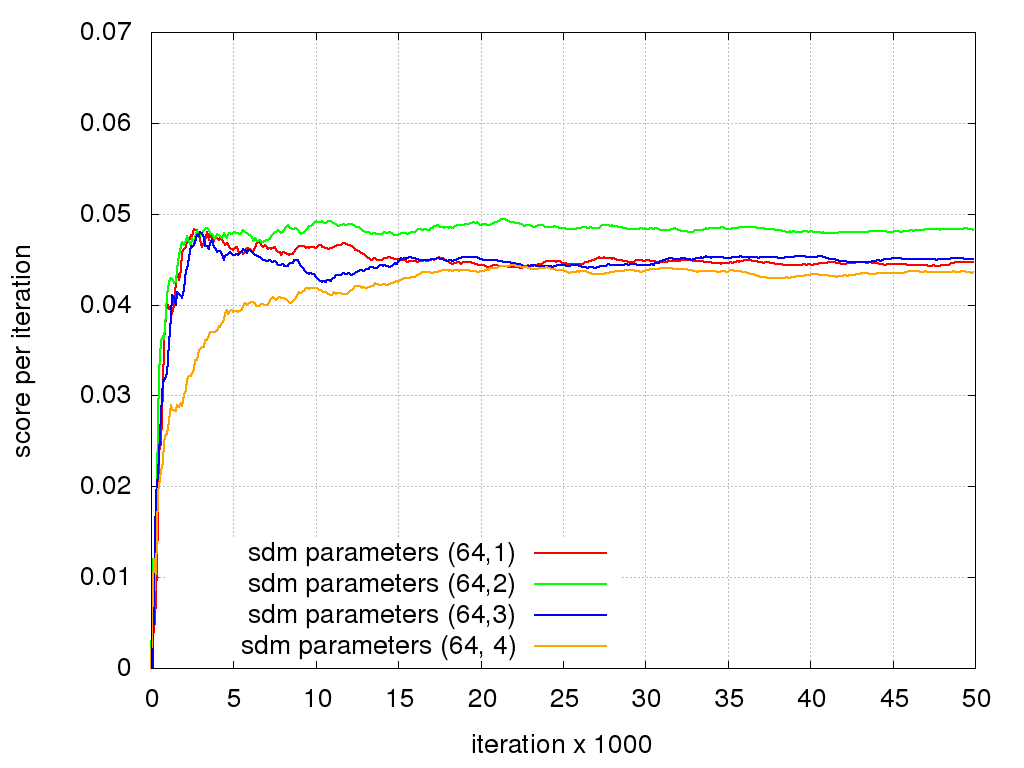
\includegraphics[width=1.0\linewidth]{{../results/worms_result/progress_experiment_/progress_per_iteration_64}.png}
\end{minipage}%
\begin{minipage}{.5\textwidth}
  \centering
  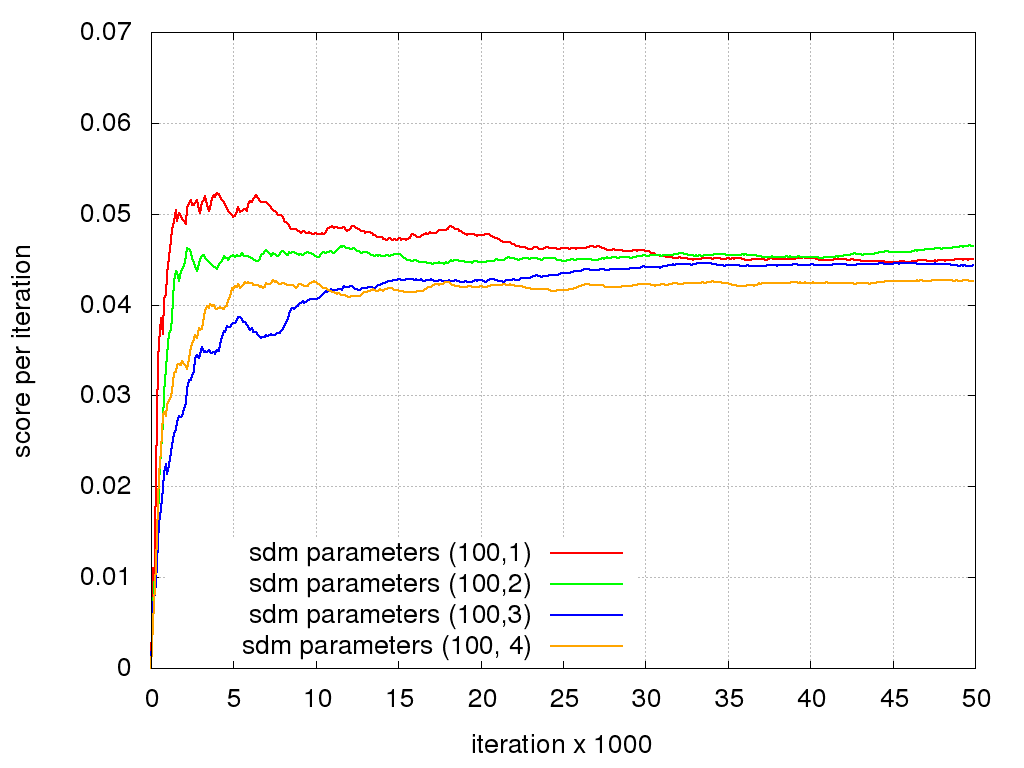
\includegraphics[width=1.0\linewidth]{{../results/worms_result/progress_experiment_/progress_per_iteration_100}.png}
\end{minipage}
\end{figure}
}
\end{frame}



\begin{frame}{\bf Line follower}

\centering
\begin{figure}[C]
   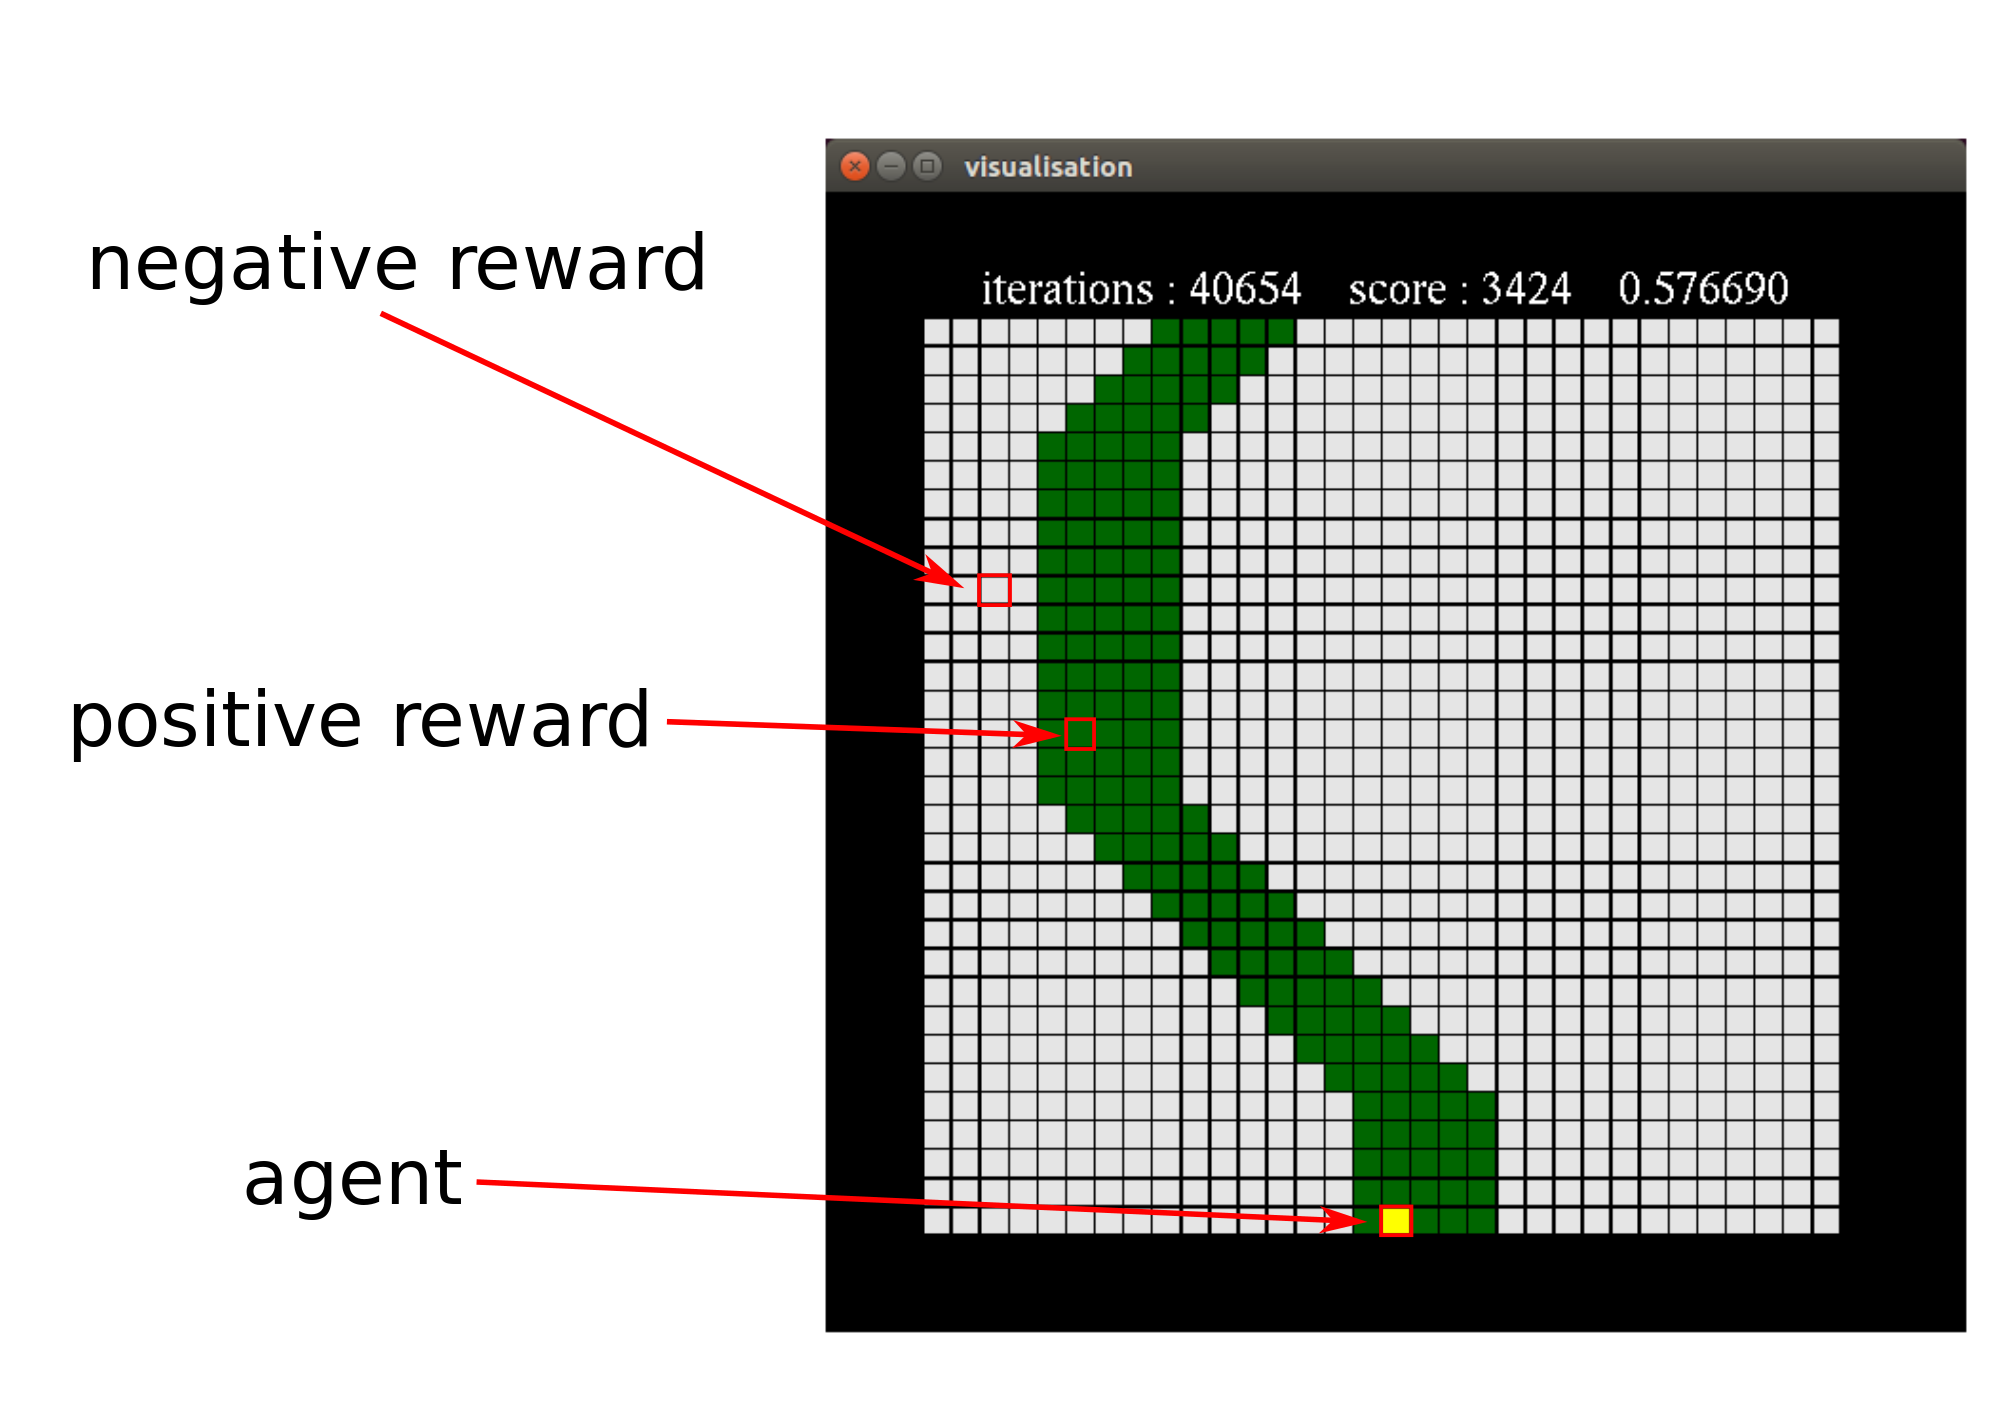
\includegraphics[scale=0.15]{../pictures/rl_race_desc.png}
\end{figure}

\end{frame}



\begin{frame}{\bf Line follower}


\begin{figure}
\centering
\begin{minipage}{.5\textwidth}

\begin{itemize}

\item motion equations of robot

\begin{align*}
a(n) &= \{-1, 0, 1\} \\
v(n) &= \alpha r(n-1) + (1.0 - \alpha) a(n) \\
p(n) &= p(n-1) + v(n)
\end{align*}

\item reward

\[
    r(n)=
\begin{cases}
    +1,& \text{if green field}\\
    -1, & \text{otherwise}
\end{cases}
\]


\end{itemize}

\end{minipage}%
\begin{minipage}{.45\textwidth}
  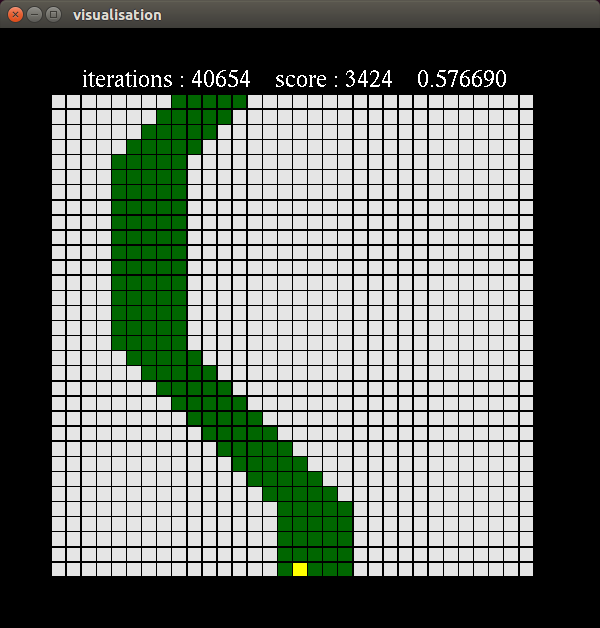
\includegraphics[scale=0.2]{../pictures/rl_race.png}
\end{minipage}
\end{figure}



\end{frame}



\begin{frame}{\bf Line follower - results}


\centering
\begin{figure}[C]
   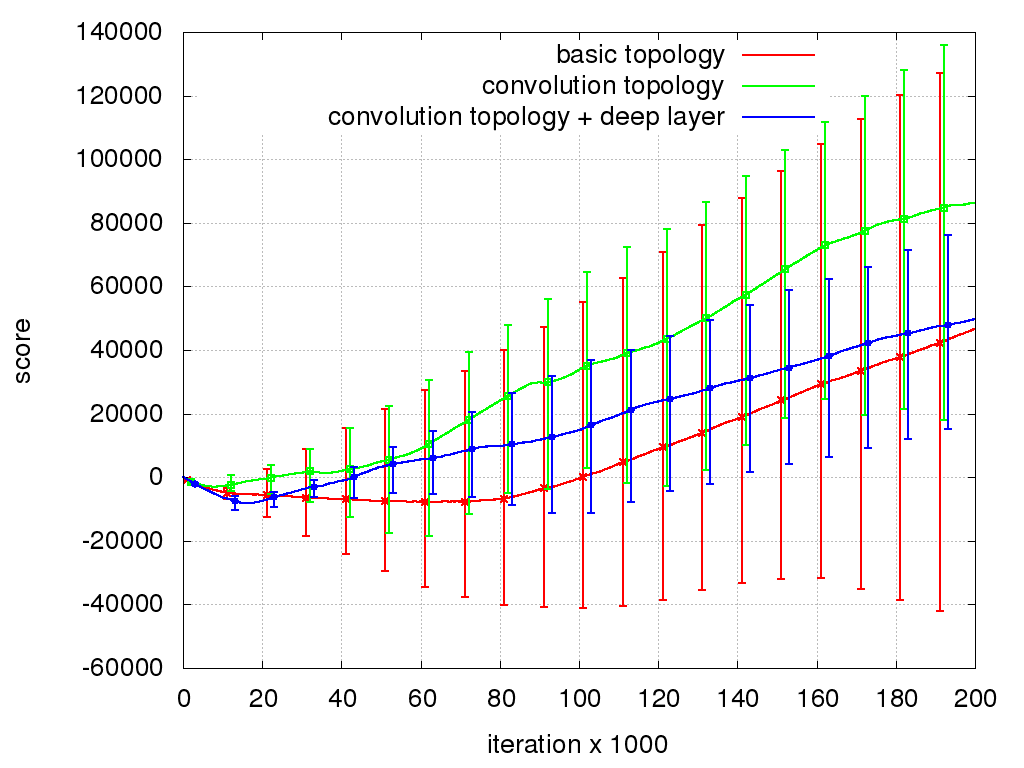
\includegraphics[scale=0.35]{../results/rl_race_experiment/deep_progress.png}
\end{figure}

\end{frame}




\begin{frame}{\bf Line follower - results}


\centering
\begin{figure}[C]
   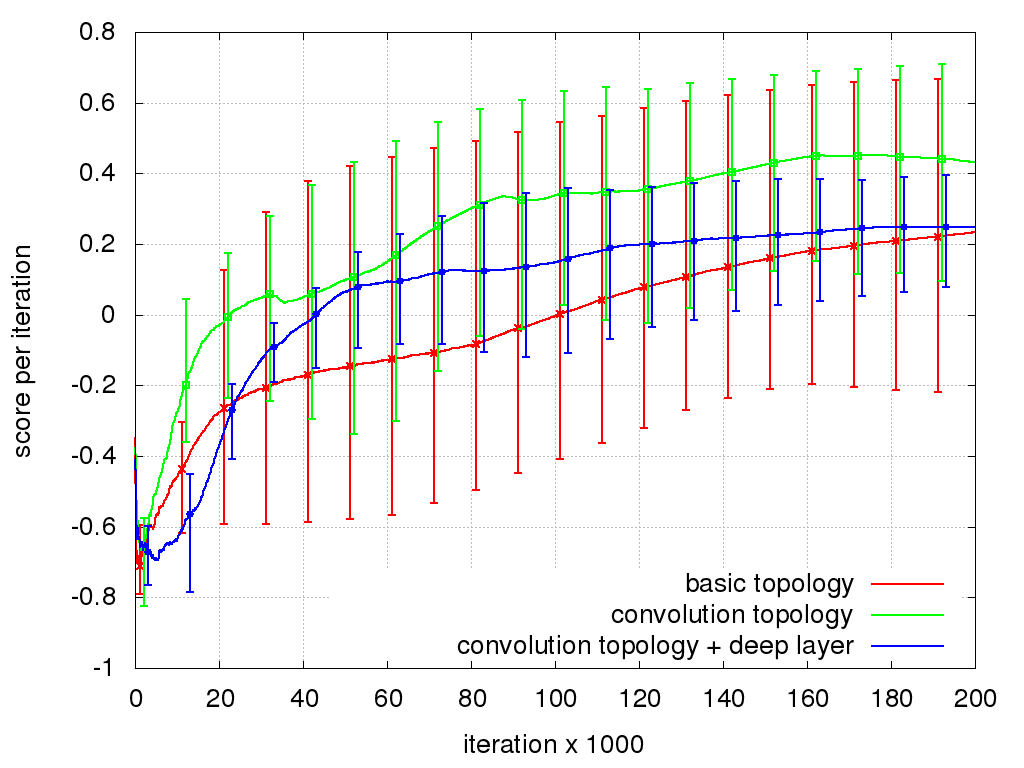
\includegraphics[scale=0.35]{../results/rl_race_experiment/deep_progress_per_iteration.png}
\end{figure}

\end{frame}

%-------------------------------------------------------------------------------------
\begin{frame}{\bf Q\&A}

\begin{figure}[ht]
\begin{center}
\begin{minipage}{0.8\linewidth}
\begin{center}
 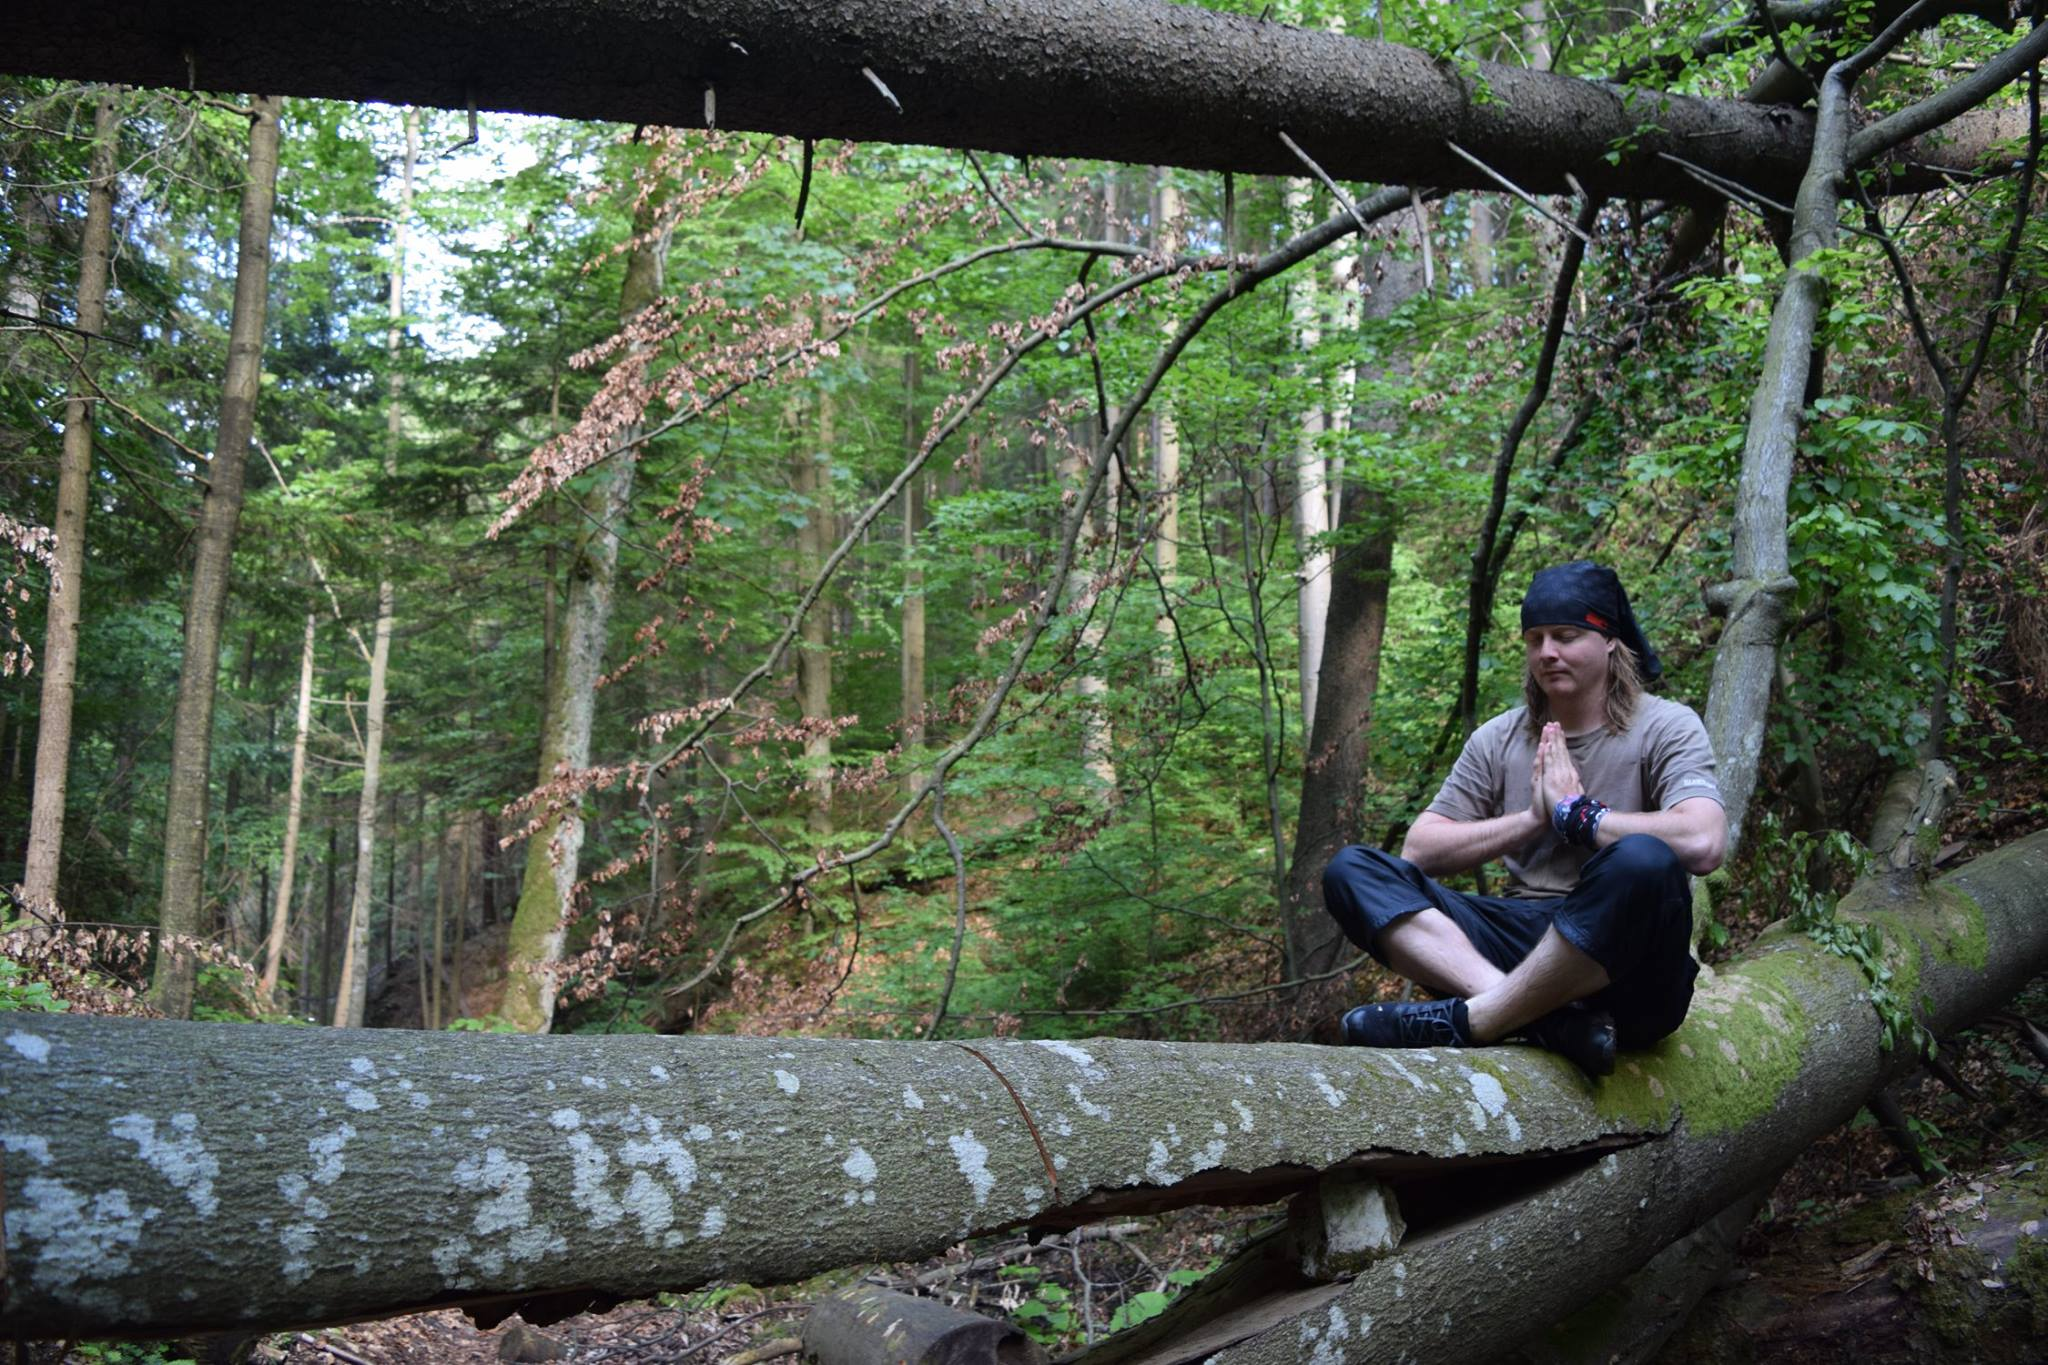
\includegraphics[width=1.0\textwidth]{../pictures/me.jpg}
\end{center}
\end{minipage}
\end{center}
\end{figure}

\url{https://github.com/michalnand/robotics}
\url{https://github.com/michalnand/machine\_learning\_new}

\centerline{michal.nand@gmail.com}

\end{frame}

\end{document}
